\documentclass[11pt,letterpaper]{article}

\usepackage{fancyhdr}
\usepackage{lastpage}
\usepackage[T1]{fontenc}
\usepackage[latin1]{inputenc}
\usepackage[cyr]{aeguill}
\usepackage[colorlinks=true]{hyperref}
\usepackage{textpos}
\usepackage{graphicx}
\usepackage[english]{babel}
\usepackage{color}
\usepackage{array}
\usepackage{enumitem}
\usepackage{amsmath}
\usepackage{amssymb}
\usepackage{amsthm}
\usepackage{multicol}   % For side-by-side formatting

\usepackage{framed}
%\usepackage{enumerate}
\definecolor{shadecolor}{gray}{0.9}

\usepackage{xcolor}

\definecolor{problemcolor}{rgb}{0.2, 0.1, 0.8} % Define color for Problem
\definecolor{solproblemcolor}{rgb}{0.8, 0.2, 0.2} % Define color for Solution to Problem

\theoremstyle{definition}
\newtheorem{prob}{\textcolor{problemcolor}{Problem}}  % Color for Problem
\newtheorem{solprob}{\textcolor{solproblemcolor}{Solution to Problem}}  % Col

\usepackage[letterpaper, left=25mm, right=25mm, top=20mm, bottom=30mm]{geometry}
\usepackage{amsmath}
\usepackage{amssymb}
\usepackage{amsfonts}
\usepackage{dsfont}
\usepackage{amsthm}
\usepackage{float}

%\usepackage{enumerate}
\usepackage{fancyhdr}
\pagestyle{fancy}

\renewcommand{\headrulewidth}{0pt}
\renewcommand{\footrulewidth}{4pt}
\allowdisplaybreaks

\newcommand{\session}{Fall 2025}




\def\0{{\mathbf 0}}
\def\1{{\mathbf 1}}

\def\a{{\mathbf a}}
\def\b{{\mathbf b}}
\def\c{{\mathbf c}}
\def\d{{\mathbf d}}
\def\e{{\mathbf e}}
\def\f{{\mathbf f}}
\def\g{{\mathbf g}}
\def\h{{\mathbf h}}
\def\i{{\mathbf i}}
\def\j{{\mathbf j}}
\def\k{{\mathbf k}}
\def\l{{\mathbf l}}
\def\m{{\mathbf m}}
\def\n{{\mathbf n}}
\def\o{{\mathbf o}}
\def\p{{\mathbf p}}
\def\q{{\mathbf q}}
\def\r{{\mathbf r}}
\def\s{{\mathbf s}}
\def\t{{\mathbf t}}
\def\u{{\mathbf u}}
\def\v{{\mathbf v}}
\def\w{{\mathbf w}}
\def\x{{\mathbf x}}
\def\y{{\mathbf y}}
\def\z{{\mathbf z}}

\def\A{{\mathbf A}}
\def\B{{\mathbf B}}
\def\C{{\mathbf C}}
\def\D{{\mathbf D}}
\def\E{{\mathbf E}}
\def\F{{\mathbf F}}
\def\G{{\mathbf G}}
\def\F{{\mathbf F}}
\def\H{{\mathbf H}}
\def\I{{\mathbf I}}
\def\J{{\mathbf J}}
\def\K{{\mathbf K}}
\def\L{{\mathbf L}}
\def\M{{\mathbf M}}
\def\N{{\mathbf N}}
\def\O{{\mathbf O}}
\def\P{{\mathbf P}}
\def\Q{{\mathbf Q}}
\def\R{{\mathbf R}}
\def\S{{\mathbf S}}
\def\T{{\mathbf T}}
\def\U{{\mathbf U}}
\def\V{{\mathbf V}}
\def\W{{\mathbf W}}
\def\X{{\mathbf X}}
\def\Y{{\mathbf Y}}
\def\Z{{\mathbf Z}}


\def\rE{{\text{E}}}
\def\rPr{{\text{Pr}}}
\def\Tr{{\text{Tr}}}
\def\vec{{\textrm{vec}}}
\def\ie{{\textit{i.e.}}}
\def\eg{{\textit{e.g.}}}


\def\cA{{\mathcal A}}
\def\cB{{\mathcal B}}
\def\cC{{\mathcal C}}
\def\cD{{\mathcal D}}
\def\cE{{\mathcal E}}
\def\cF{{\mathcal F}}
\def\cG{{\mathcal G}}
\def\cH{{\mathcal H}}
\def\cI{{\mathcal I}}
\def\cK{{\mathcal K}}
\def\cL{{\mathcal L}}
\def\cM{{\mathcal M}}
\def\cN{{\mathcal N}}
\def\cO{{\mathcal O}}
\def\cP{{\mathcal P}}
\def\cQ{{\mathcal Q}}
\def\cR{{\mathcal R}}
\def\cS{{\mathcal S}}
\def\cT{{\mathcal T}}
\def\cU{{\mathcal U}}
\def\cV{{\mathcal V}}
\def\cW{{\mathcal W}}
\def\cX{{\mathcal X}}
\def\cY{{\mathcal Y}}
\def\cZ{{\mathcal Z}}


\def\bphi{{\pmb{\phi}}}
\def\bpsi{{\pmb{\psi}}}
\def\bphi{{\pmb{\phi}}}
\def\bpsi{{\pmb{\psi}}}
\def\balpha{{\boldsymbol \alpha}}
\def\bbeta{{\boldsymbol \beta}}
\def\bvarphi{{\boldsymbol \varphi}}
\def\bPhi{{\boldsymbol \Phi}}


\def\bcdot{{\;\boldsymbol{\cdot}\;}}


%\oddsidemargin 0pt
%\topmargin 0pt
%\textwidth 6.5in
%\textheight 8.1in
\newtheorem{exemple}{Exemple}

\definecolor{bleu_poly}{RGB}{65,170,230}
\definecolor{vert_poly}{RGB}{140,200,60}
\definecolor{orange_poly}{RGB}{250,150,30}
\definecolor{rouge_poly}{RGB}{185,30,50}
\definecolor{gris_poly}{RGB}{166,168,171}

\newcommand{\matlab}{\textsc{Matlab} }
\newcommand{\simulink}{\textsc{Simulink} }

\title{\vspace{-5.5cm} \noindent\makebox[\linewidth]{\color{rouge_poly}{\rule{\textwidth}{1.5pt}}}
	\begin{center}
		\begin{tabular}{m{8cm}m{7cm}}
			\textbf{ \huge Homework 2}  & 
\includegraphics[width=0.4\textwidth]{York_logo}
		\end{tabular}
	\end{center}
	\noindent\makebox[\linewidth]{\color{rouge_poly}{\rule{\textwidth}{1.5pt}}}
	\\ \ \\
	\LARGE EECS 2200 - Electrical Circuits}\vspace{0.01mm}


\author{\session\vspace{3mm} \\ Departement of Electrical Engineering and Computer Science \\\vspace{8mm}
	York University\\
	\textbf{Instructor:} Houshang Karimi}

\date{\textbf{Due Date:} October 10, 2025\\[5mm]
	\textbf{Last Update:} \today}

\pagestyle{fancy}

\usepackage{lastpage}
%\rfoot{Page \thepage~of \pageref{LastPage}}

\lfoot{\session}
\cfoot{~~~~~~~EECS 2200 - Electrical Circuits ~~~~~~~ Page \thepage~of \pageref{LastPage}}

\chead{}
\lhead{\emph{Homework 2}}
\rhead{\includegraphics[width=3.5cm]{York_Logo}}
%\rhead{\vspace{-1cm}\includegraphics[width=2cm]{polytechnique_genie_droite_fr_cmyk}}
\renewcommand{\headrulewidth}{0.4pt}
\renewcommand{\footrulewidth}{0.4pt} 
\setlength{\headheight}{45pt}

\graphicspath{{Fig/}}

\newcounter{numq}
\setcounter{numq}{1}    % Value is 0

%\setenumerate[1]{label=(\alph*), leftmargin=3em}

\begin{document}
	\maketitle
	\vspace{-5mm}

%\noindent\makebox[\linewidth]{\color{rouge_poly}{\rule{\textwidth}{1.3pt}}}
%%%%	******************%
%\noindent\textbf{Note:} Writing your homework in \textbf{LaTeX} will be rewarded with bonus points! 

%\begin{enumerate}[label=(\roman*)]
%	\item Writing your homework in \textbf{LaTeX} will be rewarded with bonus points! 
%	\item Submit your MATLAB simulation files (.m files) along with your homework solutions. 
%\end{enumerate} 
\noindent\makebox[\linewidth]{\color{rouge_poly}{\rule{\textwidth}{1.3pt}}}	
%%%%	******************%
	
	\vspace{5mm}
	
	\centering
	\fbox{\begin{minipage}{30em}
			\vspace{4mm}
			First Name: Thomas\\\vspace{2mm}
			
			Last Name: Newman\\\vspace{2mm}
			
			Student Number: 221224662
			\vspace{3mm}
	\end{minipage}}
	
	\vspace{-0.1mm}
	
	%\centering
\begin{table}[!h]
	\centering
	\renewcommand{\arraystretch}{2.5}
	\resizebox{0.95\textwidth}{!}{ % Adjust 0.95 to a smaller value to reduce width
		\begin{tabular}{|l|l|l|l|l|l|l|l|l|l|l|l|l|l|l|l|l|l|l|}
			\cline{1-18}
			Problem		& $P_1$ & $P_2$ & $P_3$ & $P_4$  & $P_5$  & $P_6$ &  $P_7$  & $P_8$ &  $P_9$  & $P_{10}$  & $P_{11}$  &  $P_{12}$  &  $P_{13}$  &  $P_{14}$  & $P_{15}$  & $P_{16}$  &   Total  \\ \cline{1-18}
			Mark	    	&  $\dfrac{}{~5~}$ &  $\dfrac{}{~5~}$ &  $\dfrac{}{~5~}$ &  $\dfrac{}{~5~}$ & $\dfrac{}{~5~}$ & $\dfrac{}{~5~}$  & $\dfrac{}{~5~}$   & $\dfrac{}{~5~}$   & $\dfrac{}{~5~}$   & $\dfrac{}{~5~}$   & $\dfrac{}{~5~}$   & $\dfrac{}{~5~}$   &$\dfrac{}{~5~}$   &$\dfrac{}{~5~}$   &$\dfrac{}{~5~}$   & $\dfrac{}{~5~}$   &  $\dfrac{}{~80~}$ \\ \cline{1-18}
		\end{tabular}
	}
	\renewcommand{\arraystretch}{1}
\end{table}

	\noindent\makebox[\linewidth]{\color{rouge_poly}{\rule{\textwidth}{1.5pt}}}
	
\begin{enumerate}
	\item[{\textbf{CLO1:}}] \textbf{Analyze resistive circuits using basic laws (node and loop analysis, Thevenin, Norton's, superposition).}
	\item[{\textbf{CLO2:}}] \textbf{Determine the transient response of RC, RL, and RLC circuits.}
	\item[{\textbf{CLO3:}}] \textbf{Analyze AC circuits in steady state using the phasor method.}
	\item[{\textbf{CLO4:}}] \textbf{Use basic tools such as MATLAB and SPICE for circuit analysis.}
	\item[{\textbf{CLO5:}}] \textbf{Measure basic electrical signals using electronic measurement equipment in a lab setting.}
\end{enumerate}

	\noindent\makebox[\linewidth]{\color{rouge_poly}{\rule{\textwidth}{1.5pt}}}
	\newpage
%%%%%%%%%%%%%%%%%%%%%%%%%%%%%%%%%%%%%%%%%%%%%%%%%%%%%%%%%%%%%%%%%%%%%%%%%%%%%%%%%%%%%%%%%%%%%%%%%%%%%%%%%%%%%%%%%%%%%%%%%%%%%%%%%%%%%%%%%%%%%%
%%%%%%%%%%%%%%%%%%%%%%%%%%%%%%%%%%%%%%%%%%%%%%%%%%%%%%%%%%%%%%%%%%%%%%%%%%%%%%%%%%%%%%%%%%%%%%%%%%%%%%%%%%%%%%%%%%%%%%%%%%%%%%%%%%%%%%%%%%%%%%
%%%%%%%%%%%%%%%%%%%%%%%%%%%%%%%%%%%%%%%%%%%%%%%%%%%%%%%%%%%%%%%%%%%%%%%%%%%%%%%%%%%%%%%%%%%%%%%%%%%%%%%%%%%%%
%%%%%%%%%%%%%%%%%%%%%%%%%%%%%%%%%%%%%%%%%%%%%%%%%%%%%%%%%%%%%%%%%%%%%%%%%%%%%%%%%%%%%%%%%%%%%%%%%%%%%%%%%%%%%
%%%%%%%%%%%%%%%%%%%%%%%%%%%%%%%%%%%%%%%%%%%%%%%%%%%%%%%%%%%%%%%%%%%%%%%%%%%%%%%%%%%%%%%%%%%%%%%%%%%%%%%%%%%%%
%%%%%%%%%%%%%%%%%%%%%%%%%%%%%%%%%%%%%%%%%%%%%%%%%%%%%%%%%%%%%%%%%%%%%%%%%%%%%%%%%%%%%%%%%%%%%%%%%%%%%%%%%%%%%
	
%%% Alex 7th ed P2.18 and P2.35	
\begin{prob}\label{pb:p1}\text{} 
		\begin{enumerate}[label=(\alph*)]
				\item Find $I$ and $V_{ab}$ in the circuit of Fig.~\ref{fig_p1}(A).
				\item Calculate $V_o$ and $I_o$ in the circuit of Fig.~\ref{fig_p1}(B).
			\end{enumerate}
\begin{figure}[H]
	\centering
	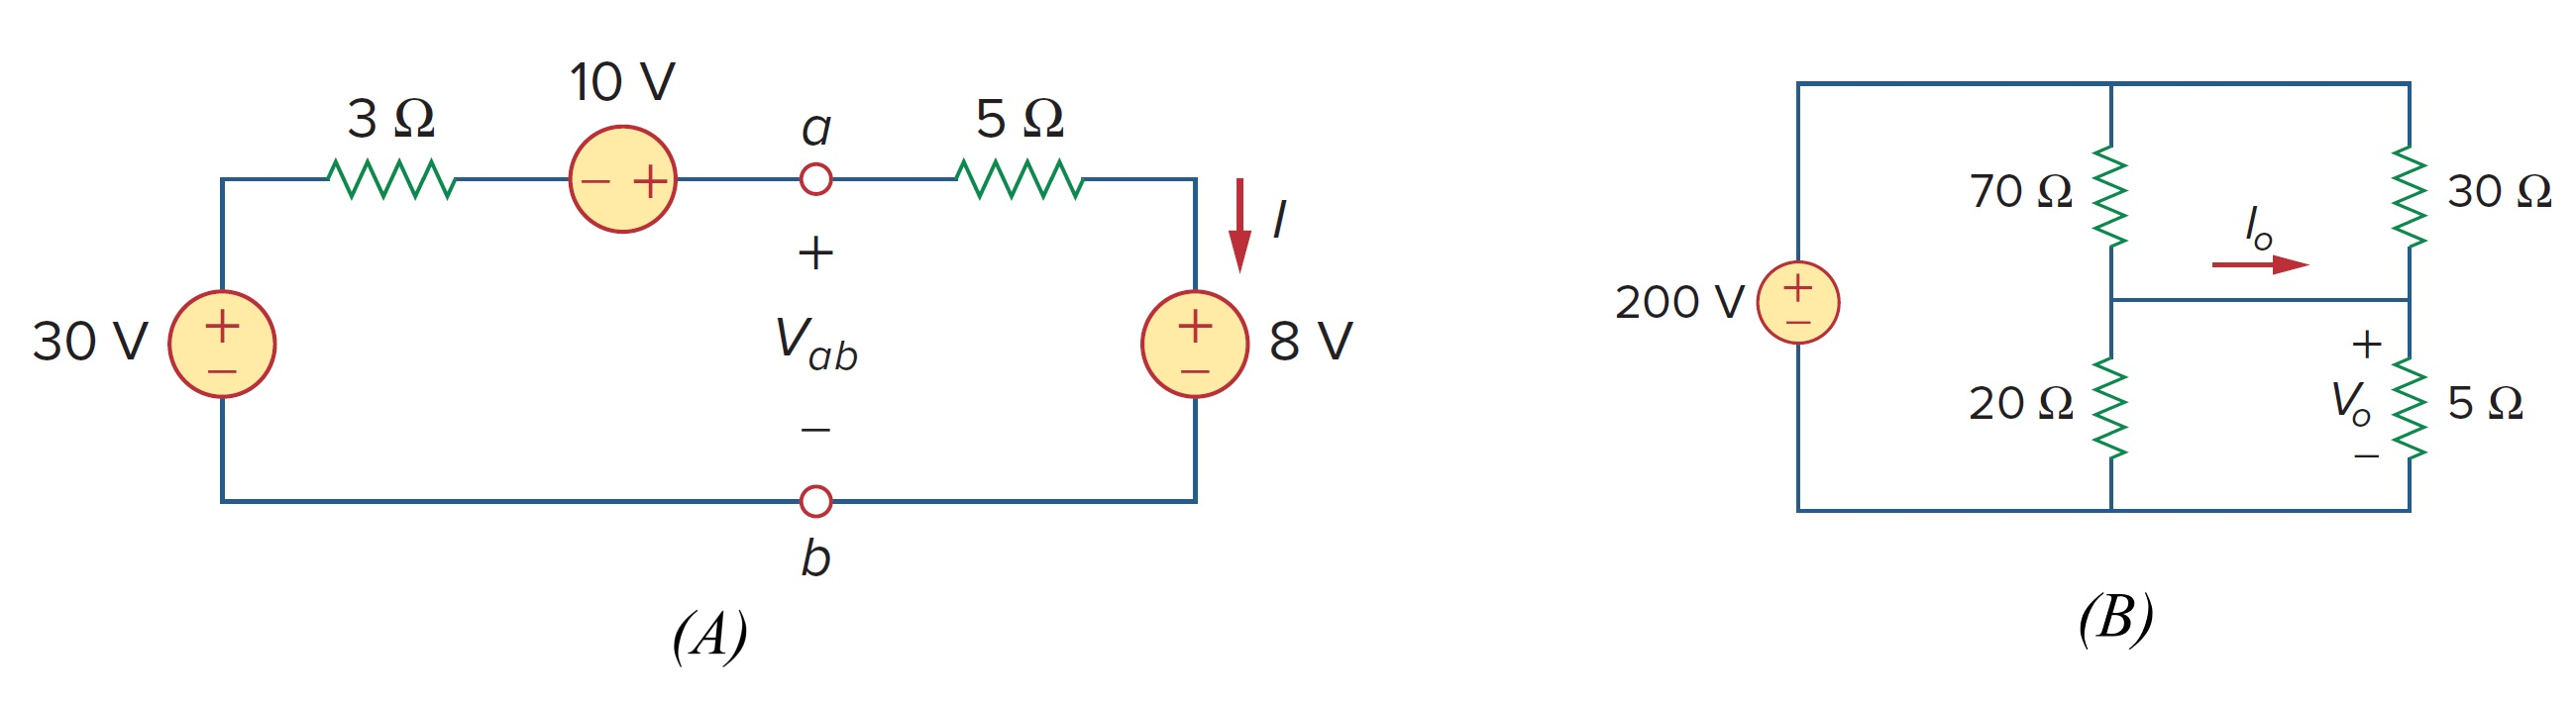
\includegraphics[width=0.8\textwidth]{Fig2.jpg}
	\caption{Circuit for Problem~\ref{pb:p1}.}
	\label{fig_p1}
\end{figure}
\end{prob}

\noindent\makebox[\linewidth]{\color{rouge_poly}{\rule{\textwidth}{1.3pt}}}

\begin{solprob} \text{}\\
    (a) We begin by using KVL around the loop.
    \[-30 + 3I -10+5I+8 = 0\]
    \[8I = 32\]
    \[I = 4 \text{ A}\]
    Now take the voltage difference from point A to point B to solve for V$_\text{ab}$.
    \[-V_\text{ab} +5I +8V = 0\]
    \[-V_\text{ab} +5(4) + 8V = 0\]
    \[V_\text{ab} = 28\text{ V}\]
    (b) Let's begin by taking the 70$\Omega$ resistor and the 30 $\Omega$ in parallel and the same with the 20 $\Omega$ resistor and the 5 $\Omega$ resistor.
    \[R_\text{eq1} = 70||30 = \frac{(70)(30)}{70+30} = 21 \Omega\]
    \[R_\text{eq2} = 5||20 = \frac{(5)(20)}{5+20} = 4\Omega\]
    \[R_\text{eq} = 21\Omega + 4\Omega = 25\Omega\]
    Now, we can solve for the current in the system using the voltage in the voltage source and the equivalent resisitance.
    \[V = IR\]
    \[I = \frac{V}{R} = \frac{200}{25} = 8 A\]
    Now, we solve for the voltage on the top and bottom of the loops.
    \[v_\text{1} = IR_\text{eq1} = (8)(21) = 168 \text{ V}\]
    \[v_\text{o} = IR_\text{eq2} = (8)(4) = 32 \text{ V}\]
    Finally, we solve for the individual currents to find $I_1$ and $I_2$.
    \[I_1 = \frac{v_1}{70\Omega} = \frac{168}{70} = 2.4A\]
    \[I_2 = \frac{v_0}{20\Omega} = \frac{32}{20} = 1.6 A\]
    At the node on the left, we take KCL to solve for $I_0$.
    \[I_1 = I_2 + I_0\]
    \[2.4A = 1.6A + I_0\]
    \[I_0 = 0.8 A\]
\end{solprob}

\noindent\makebox[\linewidth]{\color{rouge_poly}{\rule{\textwidth}{1.3pt}}}	
%%%%%%%%%%%%%%%%%%%%%%%%%%%%%%%%%%%%%%%%%%%%%%%%%%%%%%%%%%%%%%%%%%%%%%%%%%%%%%%%%%%%%%%%%%%%%%%%%%%%%%%%%%%%%%
%%%%%%%%%%%%%%%%%%%%%%%%%%%%%%%%%%%%%%%%%%%%%%%%%%%%%%%%%%%%%%%%%%%%%%%%%%%%%%%%%%%%%%%%%%%%%%%%%%%%%%%%%%%%%%
%%%%%%%%%%%%%%%%%%%%%%%%%%%%%%%%%%%%%%%%%%%%%%%%%%%%%%%%%%%%%%%%%%%%%%%%%%%%%%%%%%%%%%%%%%%%%%%%%%%%%%%%%%%%%%
%%%%%%%%%%%%%%%%%%%%%%%%%%%%%%%%%%%%%%%%%%%%%%%%%%%%%%%%%%%%%%%%%%%%%%%%%%%%%%%%%%%%%%%%%%%%%%%%%%%%%%%%%%%%%%
%%% Alex 7th ed P2.18 and P2.39
\begin{prob}\label{pb:p2} Evaluate $R_{eq}$ looking into each set of terminals for each of the circuits shown in Fig.~\ref{fig_Req1}.

\begin{figure}[H]
	\centering
	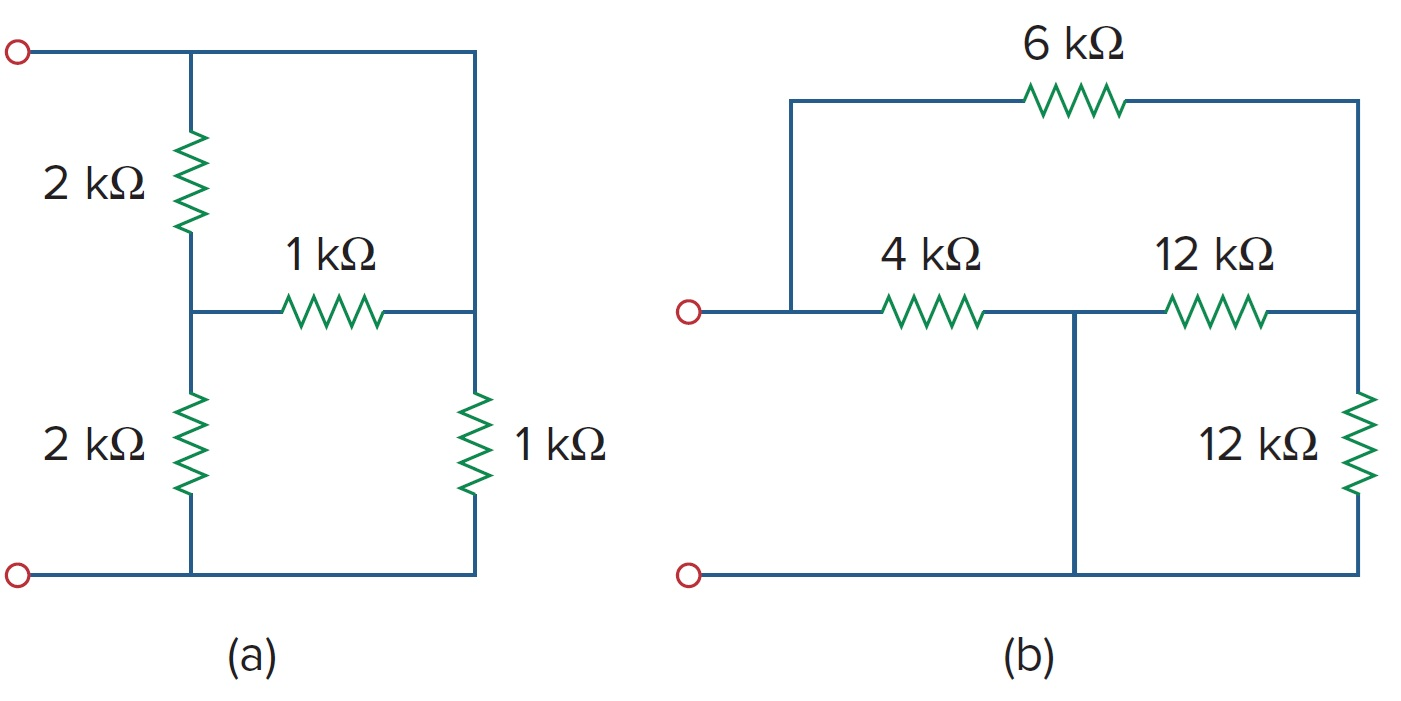
\includegraphics[width=0.5\textwidth]{Fig3.jpg}
	\caption{Circuit for Problem~\ref{pb:p2}.}
	\label{fig_Req1}
\end{figure}

\end{prob}

\noindent\makebox[\linewidth]{\color{rouge_poly}{\rule{\textwidth}{1.3pt}}}

\begin{solprob} \text{}\\
    (a) Let's begin by combining the 2k$\Omega$ and the 1k$\Omega$ in parallel.
    \[R_\text{eq1} = 2||1 = \frac{(2)(1)}{2+1} = \frac{2}{3}k\Omega\]
    Now combine the $\frac{2}{3}\text{k}\Omega$ resistor with the second $2\text{k}\Omega$ resistor.
    \[R_\text{eq2} = \frac{2}{3} + 2 = \frac{8}{3}k\Omega\]
    Now solve for the final $R_\text{eq}$.
    \[R_\text{eq} = \frac{8}{3}k\Omega || 1k\Omega = \frac{(\frac{8}{3}k\Omega)(1k\Omega)}{\frac{11}{3}k\Omega} = 727.29\Omega\]
    (b) Let's begin by combining the 2 $12k\Omega$ resistors in parallel.
    \[R_\text{eq1} = 12k\Omega||12k\Omega = \frac{(12)(12)}{12 + 12} = 6k\Omega\]
    Now let's combine the $6k\Omega$ resistor in series with this new one.
    \[R_\text{eq2} = 6k\Omega + 6k\Omega = 12k\Omega\]
    Finally, lets calculate the $R_\text{eq}$ of the circuit.
    \[R_\text{eq} = 12k\Omega||4k\Omega = \frac{(12)(4)}{12 + 4} = 3k\Omega\]
\end{solprob}

\noindent\makebox[\linewidth]{\color{rouge_poly}{\rule{\textwidth}{1.3pt}}}	
%%%%%%%%%%%%%%%%%%%%%%%%%%%%%%%%%%%%%%%%%%%%%%%%%%%%%%%%%%%%%%%%%%%%%%%%%%%%%%%%%%%%%%%%%%%%%%%%%%%%%%%%%%%%%%
%%%%%%%%%%%%%%%%%%%%%%%%%%%%%%%%%%%%%%%%%%%%%%%%%%%%%%%%%%%%%%%%%%%%%%%%%%%%%%%%%%%%%%%%%%%%%%%%%%%%%%%%%%%%%%
%%%%%%%%%%%%%%%%%%%%%%%%%%%%%%%%%%%%%%%%%%%%%%%%%%%%%%%%%%%%%%%%%%%%%%%%%%%%%%%%%%%%%%%%%%%%%%%%%%%%%%%%%%%%%%
%%%%%%%%%%%%%%%%%%%%%%%%%%%%%%%%%%%%%%%%%%%%%%%%%%%%%%%%%%%%%%%%%%%%%%%%%%%%%%%%%%%%%%%%%%%%%%%%%%%%%%%%%%%%%%
%% Alex 7th ed P2.47
\begin{prob}\label{pb:p3}
	Find the equivalent resistance $R_{ab}$ in the circuits of Fig.~\ref{fig_Req2}.
\end{prob}

\begin{figure}[H]
	\centering
	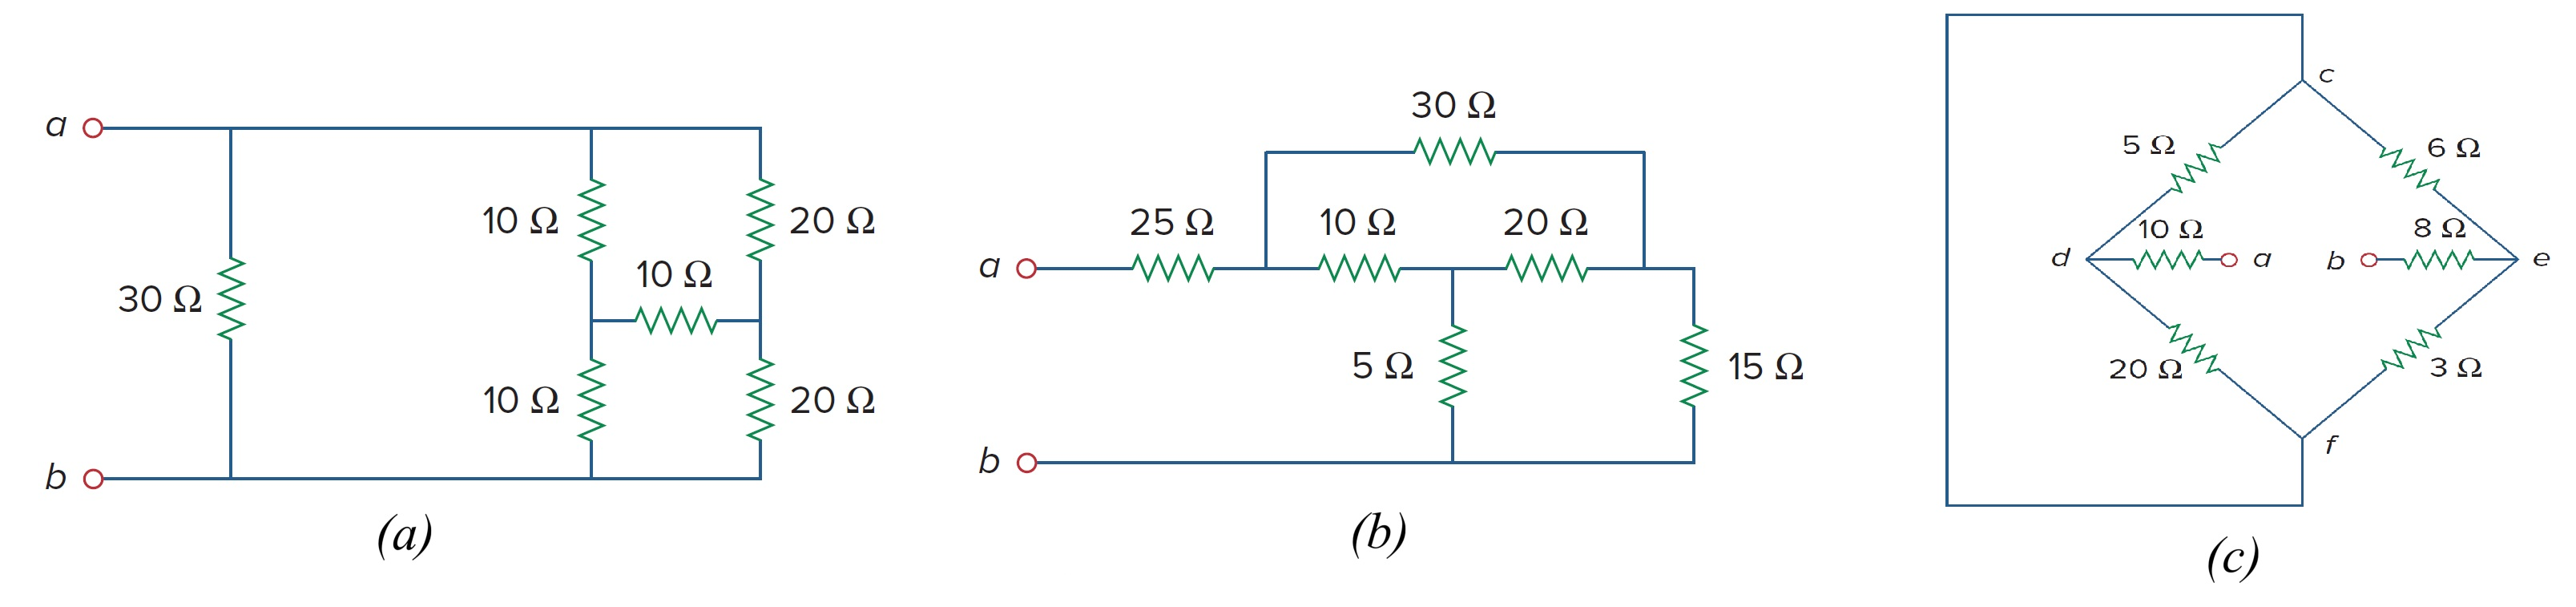
\includegraphics[width=0.95\textwidth]{Fig4.jpg}
	\caption{Circuit for Problem~\ref{pb:p3}.}
	\label{fig_Req2}
\end{figure}

\noindent\makebox[\linewidth]{\color{rouge_poly}{\rule{\textwidth}{1.3pt}}}

\begin{solprob} \text{}\\
    (a) Let's begin by performing a Wye-to-Delta transformation on the left node of the far right side of the circuit.
    \[R_1 = 10\Omega \,\,\,\,\,\, R_2 = 10\Omega\,\,\,\,\,\, R_3 = 10\Omega\]
    Let's form the delta resistors, $R_a$, $R_b$, $R_c$.
    \[R_a = R_b = R_c = \frac{10(10) + 10(10) + 10(10)}{10} = 30\Omega\]
    Now, lets combine the top and bottom 20$\Omega$ resistors in parallel with two of the 30$\Omega$ resistors.
    \[R_\text{eq1} = 30||20 = \frac{(30)(20)}{30 + 20} = 12\Omega\]
    Now we combine them in series.
    \[R_\text{eq2} = 12\Omega + 12\Omega = 24\Omega\]
    Finally, we finish by combining the 2 remaining 30$\Omega$ resistors and the 24$\Omega$ resistor in parallel.
    \[R_\text{eq} = 30||30||24 = \frac{(\frac{(30)(30)}{30 + 30})(24)}{\frac{(30)(30)}{30 + 30}+24} = 9.23\Omega\]
    (b) Let's begin by selecting the center node connected to the $10\Omega$, $20\Omega$ and the $5\Omega$ resistors and performing a Wye-to-Delta transformation.
    \[R_1 = 10\Omega \,\,\,\,\,\, R_2 = 20\Omega\,\,\,\,\,\, R_3 = 5\Omega\]
    Now we calculate the delta resistors.
    \[R_\text{ab} = \frac{10(20) + 20(50) + 10(5)}{5} = 70\Omega\]
    \[R_\text{bc} \frac{10(20) + 20(50) + 10(5)}{10} = 35\Omega\]
    \[R_\text{ac} \frac{10(20) + 20(50) + 10(5)}{20} = 17.5\Omega\]
    Now, let's combine the bottom right $15\Omega$ resistor with the $35\Omega$ resistor in the delta, and the top $30\Omega$ resistor with the $70\Omega$ resistor in the delta.
    \[R_\text{eq1} = 35||15 = \frac{(35)(15)}{35+15} = 10.5\Omega\]
    \[R_\text{eq2} = 30||70 = \frac{(30)(70)}{30 + 70} = 21\Omega\]
    These two resistors are now in series, so lets combine them.
    \[R_\text{eq3} = 21 + 10.5 = 31.5\Omega\]
    Lets combine this resistor with the final delta resistor in parallel.
    \[R_\text{eq4} = 31.5||17.5 = \frac{(17.5)(31.5)}{17.5 + 31.5} = 11.25\Omega\]
    Now, lets calculate our final $R_\text{eq}$ by combining the 11.25$\Omega$ resistor with the 25$\Omega$ resistor in series.
    \[R_\text{eq} = 25 + 11.25 = 36.25\Omega\]
    (c) Let's begin by noticing that the $5\Omega$ and the $20\Omega$ resistors are in parallel, as well as the $6\Omega$ and the $3\Omega$ resistors.  Let's combine these first.
    \[R_\text{eq1} = 20||5 = \frac{(20)(5)}{20+5} = 4\Omega\]
    \[R_\text{eq2} = 6||3 = \frac{(6)(3)}{6+3} = 2\Omega\]
    This leaves us with a very simple series circuit, so let's just combine them all at once to calculate our equivalent resistance.
    \[R_\text{eq} = 10 + 8 + 4 + 2 = 24\Omega\]
\end{solprob}

\noindent\makebox[\linewidth]{\color{rouge_poly}{\rule{\textwidth}{1.3pt}}}	
%%%%%%%%%%%%%%%%%%%%%%%%%%%%%%%%%%%%%%%%%%%%%%%%%%%%%%%%%%%%%%%%%%%%%%%%%%%%%%%%%%%%%%%%%%%%%%%%%%%%%%%%%%%%%%
%%%%%%%%%%%%%%%%%%%%%%%%%%%%%%%%%%%%%%%%%%%%%%%%%%%%%%%%%%%%%%%%%%%%%%%%%%%%%%%%%%%%%%%%%%%%%%%%%%%%%%%%%%%%%%
%%%%%%%%%%%%%%%%%%%%%%%%%%%%%%%%%%%%%%%%%%%%%%%%%%%%%%%%%%%%%%%%%%%%%%%%%%%%%%%%%%%%%%%%%%%%%%%%%%%%%%%%%%%%%%
%%%%%%%%%%%%%%%%%%%%%%%%%%%%%%%%%%%%%%%%%%%%%%%%%%%%%%%%%%%%%%%%%%%%%%%%%%%%%%%%%%%%%%%%%%%%%%%%%%%%%%%%%%%%%%

%% Alex 7th ed P2.52
\begin{prob}\label{pb:p4} For the circuit shown in Fig.~\ref{fig_Req3}, find the equivalent resistance. All resistors are $3~\Omega$.

\begin{figure}[H]
	\centering
	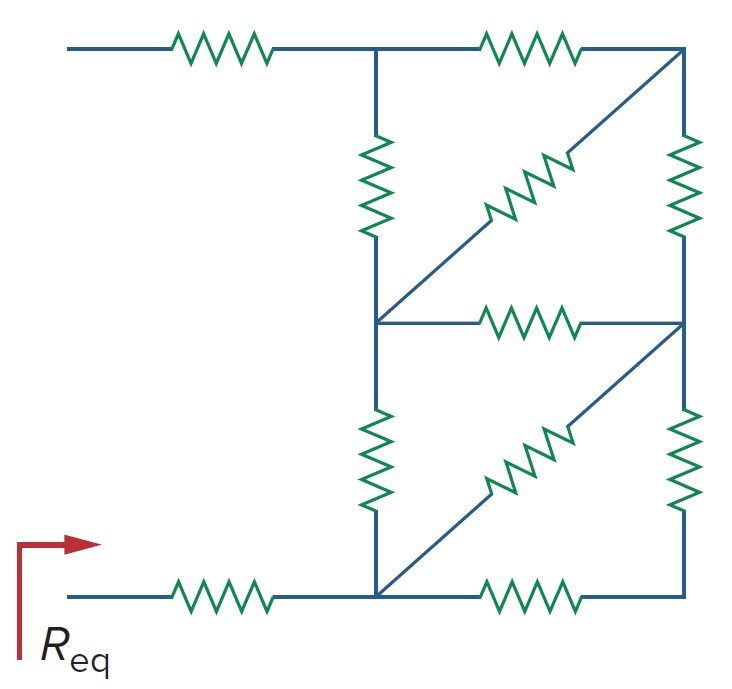
\includegraphics[width=0.35\textwidth]{Fig5.jpg}
	\caption{Circuit for Problem~\ref{pb:p4}.}
	\label{fig_Req3}
\end{figure}
\end{prob}

\noindent\makebox[\linewidth]{\color{rouge_poly}{\rule{\textwidth}{1.3pt}}}

\begin{solprob} \text{}\\
    Let's begin by combining two bottom resistors in series.
    \[R_\text{eq1} = 3 + 3 = 6\Omega\]
    Now, combine this resistor with the diagonal $3\Omega$ resistor in parallel.
    \[R_\text{eq2} = 3||6 = \frac{(3)(6)}{3+6} = 2\Omega\]
    Now, convert the very bottom node connecting the $3\Omega$, $2\Omega$ and the $3\Omega$ resistors together using a Wye-to-Delta transformation.
    \[R_1 = 2\Omega \,\,\,\,\,\, R_2 = 3\Omega\,\,\,\,\,\, R_3 = 3\Omega\]
    Now convert them to their delta values.
    \[R_\text{ab} = \frac{2(3) + 2(3) + 3(3)}{3} = 7\Omega = R_\text{ac}\]
    \[R_\text{bc} \frac{2(3) + 2(3) + 3(3)}{2} = \frac{21}{2}\Omega\]
    Now, combine the $\frac{21}{2}\Omega$ and the $7\Omega$ resistors in series, then combine it with the $7\Omega$ resistor, and then again with the straight $3\Omega$ resistor.
    \[R_\text{eq3} = \frac{21}{2}\Omega + 7\Omega = \frac{35}{2}\Omega\]
    \[R_\text{eq4} = \frac{35}{2}||7 = \frac{(\frac{35}{2})(7)}{\frac{35}{2} + 7} = 5\Omega\]
    \[R_\text{eq5} = 5||3 = \frac{(5)(3)}{5+3} = 1.875\Omega\]
    Now, we just combine this resistor with the $3\Omega$ one next to it in series, combine it with the final diagonal resistor in parallel, then in series with the top $3\Omega$ resistor, and one more time with the straight up $3\Omega$ resistor.
    \[R_\text{eq6} = 1.875 + 3 = 4.875\Omega\]
    \[R_\text{eq7} = 4.875||3 = \frac{(4.875)(3)}{4.875+3} = 1.857\Omega\]
    \[R_\text{eq8} = 1.857 + 3 = 4.857\Omega\]
    \[R_\text{eq9} = 4.857||3 = \frac{(4.857)(3)}{4.857+3} = 1.854\Omega\]
    Finally, we solve for $R_\text{eq}$ using a series connection between this resistor and the final $3\Omega$ resistor.
    \[R_\text{eq} = 1.854 + 3 = 4.85\Omega\]
\end{solprob}

\noindent\makebox[\linewidth]{\color{rouge_poly}{\rule{\textwidth}{1.3pt}}}	
%%%%%%%%%%%%%%%%%%%%%%%%%%%%%%%%%%%%%%%%%%%%%%%%%%%%%%%%%%%%%%%%%%%%%%%%%%%%%%%%%%%%%%%%%%%%%%%%%%%%%%%%%%%%%%
%%%%%%%%%%%%%%%%%%%%%%%%%%%%%%%%%%%%%%%%%%%%%%%%%%%%%%%%%%%%%%%%%%%%%%%%%%%%%%%%%%%%%%%%%%%%%%%%%%%%%%%%%%%%%%
%%%%%%%%%%%%%%%%%%%%%%%%%%%%%%%%%%%%%%%%%%%%%%%%%%%%%%%%%%%%%%%%%%%%%%%%%%%%%%%%%%%%%%%%%%%%%%%%%%%%%%%%%%%%%%
%%%%%%%%%%%%%%%%%%%%%%%%%%%%%%%%%%%%%%%%%%%%%%%%%%%%%%%%%%%%%%%%%%%%%%%%%%%%%%%%%%%%%%%%%%%%%%%%%%%%%%%%%%%%%%
% Nilsson 12th ed P1.31
\begin{prob}\label{pb:p5} Find $R_{eq}$ and $I$ in the circuit of Fig.~\ref{fig_Req4}.

\begin{figure}[H]
	\centering
	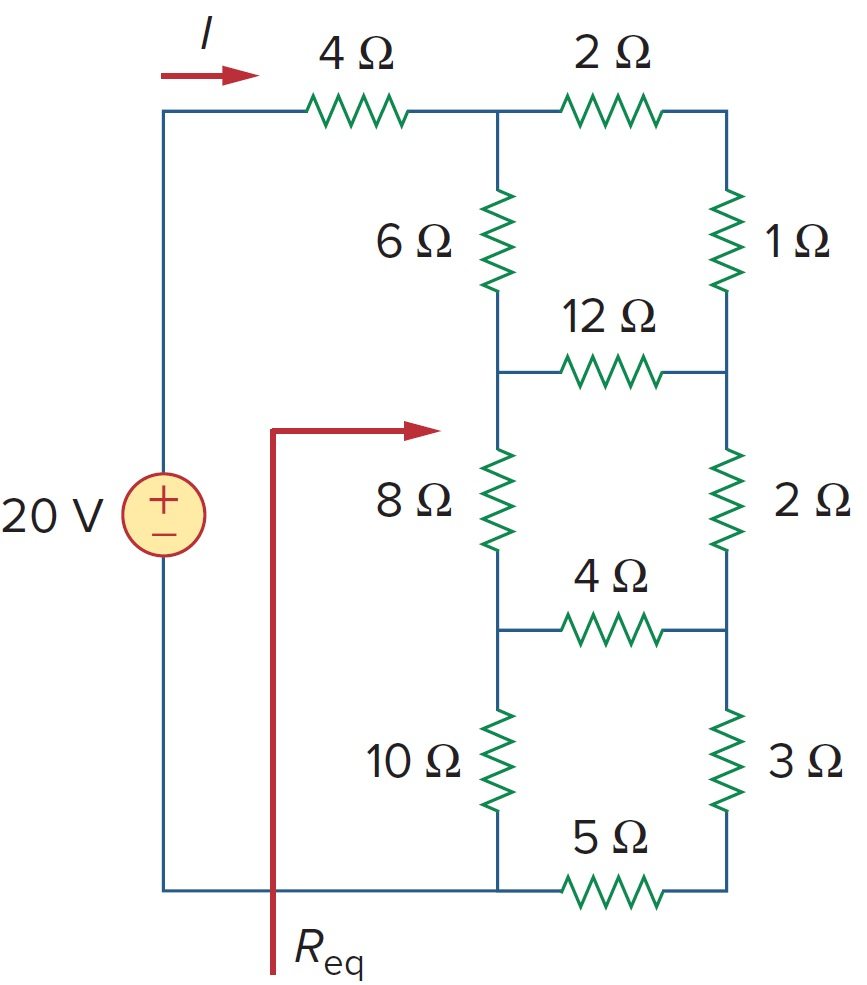
\includegraphics[width=0.35\textwidth]{Fig6.jpg}
	\caption{Circuit for Problem~\ref{pb:p5}.} 
	\label{fig_Req4}
\end{figure}
\end{prob}

\noindent\makebox[\linewidth]{\color{rouge_poly}{\rule{\textwidth}{1.3pt}}}

\begin{solprob} \text{}\\
    Let's begin by combining the top right corner and the top left corner resistors in series.
    \[R_\text{eq1} = 5 + 3 = 8\Omega\]
    \[R_\text{eq2} = 2+1 = 3\Omega\]
    Now, we will do 2 seperate Wye-to-Delta transformations in the middle portion of the circuit, one on the top left central node, and the other on the bottom right central node.
    For the first one:
    \[R_11 = 8\Omega \,\,\,\,\,\, R_21 = 6\Omega\,\,\,\,\,\, R_31 = 12\Omega\]
    Now convert them to their delta values.
    \[R_\text{ab1} = \frac{8(6) + 6(12) + 8(12)}{12} = 18\Omega\]
    \[R_\text{ac1} = \frac{8(6) + 6(12) + 8(12)}{6} = 36\Omega\]
    \[R_\text{bc1} \frac{8(6) + 6(12) + 8(12)}{8} = 27\Omega\]
    For the second one:
    \[R_12 = 2\Omega \,\,\,\,\,\, R_22 = 8\Omega\,\,\,\,\,\, R_32 = 4\Omega\]
    Now convert them to their delta values.
    \[R_\text{ab2} = \frac{2(8) + 8(4) + 2(4)}{4} = 14\Omega\]
    \[R_\text{ac2} = \frac{2(8) + 8(4) + 2(4)}{8} = 7\Omega\]
    \[R_\text{bc2} \frac{2(8) + 8(4) + 2(4)}{2} = 28\Omega\]
    This will result in the two triangles facing in opposite directions, and one resistor on each will join in parallel, in this case, its the $36\Omega$ and the $27\Omega$ are in parallel.
    \[R_\text{eq3} = 36||7 = \frac{(36)(7)}{36+7} = 5.86\Omega\]
    Also, because of our transformations, there are now 2 other resistors in parallel too, details outlined below:
    \[R_\text{eq4} = 27||3 = \frac{(27)(3)}{27+3} = 2.7\Omega\]
    \[R_\text{eq5} 28||10 = \frac{(28)(10)}{28+10} = 7.368\Omega\]
    Now, we need to make a Pi-to-Delta transformation before we can finish this circuit.
    \[R_a = \frac{R_aR_c}{R_a+R_b+R_c} = \frac{(2.7)(5.868)}{18+2.7+5.86} = 0.5957\Omega\]
    \[R_b = \frac{(5.868)(18)}{26.56} = 3.97\Omega\]
    \[R_c = \frac{(18)(2.7)}{26.56} = 1.83\Omega\]
    Now, we have a Wye-looking circuit with an extended series resistor at the end of each wire. Let's combine these and then combine them in parallel.  The final step for $R_\text{eq}$ would then be to combine the last resistors in series.
    \[R_\text{eq6} = 14+0.5957 = 14.5957\Omega\]
    \[R_\text{eq7} = 3.97 + 7.36 = 11.33\Omega\]
    \[R_\text{eq8} = 14.5957||11.33 = \frac{(14.5957)(11.33)}{14.5957 + 11.33} = 6.378\Omega\]
    \[R_\text{eq} = 6.378 + 1.83 + 4 = 12.2\Omega\]
    Now, since we have the fully simplified circuit, we can calculate for the current in the circuit using the source.
    \[I = \frac{V}{R_\text{eq}} = \frac{20}{12.2} = 1.64 A\]
\end{solprob}

\noindent\makebox[\linewidth]{\color{rouge_poly}{\rule{\textwidth}{1.3pt}}}	
%%%%%%%%%%%%%%%%%%%%%%%%%%%%%%%%%%%%%%%%%%%%%%%%%%%%%%%%%%%%%%%%%%%%%%%%%%%%%%%%%%%%%%%%%%%%%%%%%%%%%%%%%%%%%%
%%%%%%%%%%%%%%%%%%%%%%%%%%%%%%%%%%%%%%%%%%%%%%%%%%%%%%%%%%%%%%%%%%%%%%%%%%%%%%%%%%%%%%%%%%%%%%%%%%%%%%%%%%%%%%
%%%%%%%%%%%%%%%%%%%%%%%%%%%%%%%%%%%%%%%%%%%%%%%%%%%%%%%%%%%%%%%%%%%%%%%%%%%%%%%%%%%%%%%%%%%%%%%%%%%%%%%%%%%%%%
%%%%%%%%%%%%%%%%%%%%%%%%%%%%%%%%%%%%%%%%%%%%%%%%%%%%%%%%%%%%%%%%%%%%%%%%%%%%%%%%%%%%%%%%%%%%%%%%%%%%%%%%%%%%%%
%% Dorf 9th ed P3.8-6
\begin{prob}\label{pb:p6}\text{}
	\begin{enumerate}[label=(\alph*)]
		\item Use the node-voltage method to determine the branch currents $i_a$ and $i_b$ in the circuit shown in Fig.~\ref{fig_1_5}.
		\item Verify your results by showing that the total power dissipated in the circuit equals the total power supplied.
	\end{enumerate}
	
	\begin{figure}[H]
		\centering
		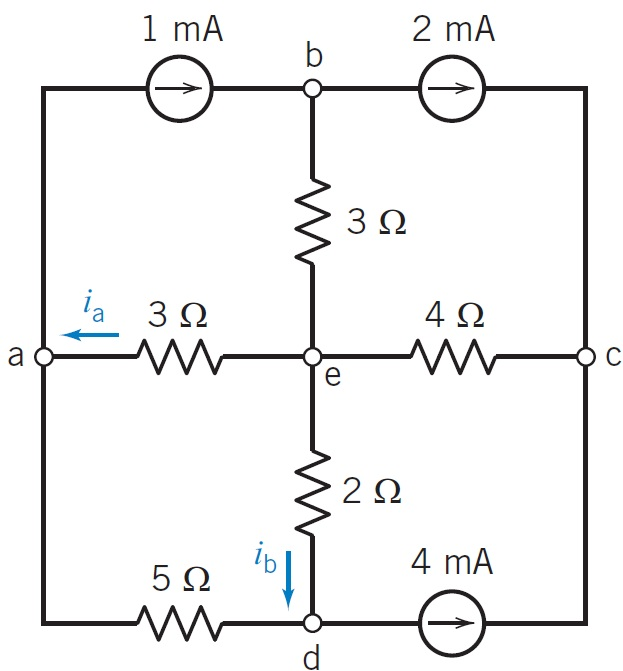
\includegraphics[width=0.33\textwidth]{Fig1.jpg}
		\caption{Circuit for Problem~\ref{pb:p6}.}
		\label{fig_1_5}
	\end{figure}
\end{prob}

\noindent\makebox[\linewidth]{\color{rouge_poly}{\rule{\textwidth}{1.3pt}}}

\begin{solprob} \text{}\\
    Let's begin by using the writing the node-voltage equations for each node.
    \[\text{Ground Node: } \frac{-V_a}{5}+\frac{-V_e}{2} + 4 = 0 \implies \frac{-V_a}{5} = \frac{V_e}{2} + 4 \implies V_a = -\frac{5}{2}V_e + 20\]
    \[\text{Node B: } \frac{V_b-V_e}{3} + 2 - 1 = 0 \implies V_b-V_e = -3 \implies V_b = -3 + V_e\]
    \[\text{Node E: } \frac{V_e-V_b}{3} + \frac{V_e-V_c}{4} + \frac{V_e-V_a}{3} + \frac{V_e}{2} = 0\]
    \[\text{Node C: } \frac{V_c - V_e}{4} -2 -4 = 0 \implies V_c-V_e = 24 \implies V_c = V_e + 24\]
    Now, substitute each equation into Node E:
    \[\frac{V_e-(-3-V_e)}{3} + \frac{V_e-(V_e+24)}{4} + \frac{V_e-(\frac{5}{2}V_e + 20)}{3} + \frac{V_e}{2} = 0\]
    \[\frac{3}{3} - \frac{24}{4} + \frac{\frac{7}{2}V_e}{3} + \frac{V_e}{2} = 0\]
    \[\frac{10}{6}V_e = 1-\frac{20}{3}-6\]
    \[V_e = 7.0mV\]
    Now solve for the remaining voltages, $V_a, V_b, V_c$.
    \[V_a = -\frac{5}{2}(7) + 20 = 2.5mV\]
    \[V_b = -3 + (7) = 4.0mV\]
    \[V_c = V_e + 24 = 7+24 = 31.0mV\]
    \[V_d = 0mV\]
    Now, solve for $i_a$ and $i_b$ using the voltage difference over the wire.
    \[i_a = \frac{V_e-V_a}{3} = \frac{7-2.5}{3} = \frac{4.5}{3}mA = 1.5mA\]
    \[i_b = \frac{V_e-V_d}{2} = \frac{V_e}{2} = \frac{7}{2}mA = 3.5mA\]
    (b) Let's calculate the power supplied vs the power dissipated.
    \[P_\text{1mA} = (V_a-V_b)i = (2.5-4.0)(1) = -1.5 \text{ $\mu$W}\]
    \[P_\text{2mA} = (V_b-V_c)i = (4.0-31.0)(2) = -54 \text{ $\mu$W}\]
    \[P_\text{4mA} = (V_d-V_c)i = (0.0-31.0)(4) = -124 \text{ $\mu$W}\]
    Total power sourced is $P_\text{total} = -1.5 - 54 - 124 = -179.5 \mu$W\newline
    Now, lets calculate the total power dissipated by the resistors.
    \[P_\text{2$\Omega$} = (i_\text{ed})^2(2) = (3.5)^2(2) = 24.5 \,\mu\text{W}\]
    \[P_\text{3$\Omega$L} = (i_\text{ae})^2(3) = (1.5)^2(3) = 6.75 \,\mu\text{W}\]
    \[P_\text{3$\Omega$T} = (i_\text{be})^2(3) = (-1)^2(3) = 3 \,\mu\text{W}\]
    \[P_\text{4$\Omega$} = (i_\text{ec})^2(4) = (6)^2(4) = 144 \,\mu\text{W}\]
    \[P_\text{5$\Omega$} = (i_\text{ad})^2(5) = (0.5)^2(5) = 1.25 \,\mu\text{W}\]
    Total power dissipated is $P_\text{dissipated} = 24.5 + 6.75 + 3 + 144 + 1.25 = 179.5\,\mu$W.\newline
\end{solprob}

\vspace{-5mm}

\noindent\makebox[\linewidth]{\color{rouge_poly}{\rule{\textwidth}{1.3pt}}}	
%%%%%%%%%%%%%%%%%%%%%%%%%%%%%%%%%%%%%%%%%%%%%%%%%%%%%%%%%%%%%%%%%%%%%%%%%%%%%%%%%%%%%%%%%%%%%%%%%%%%%%%%%%%%%%
%%%%%%%%%%%%%%%%%%%%%%%%%%%%%%%%%%%%%%%%%%%%%%%%%%%%%%%%%%%%%%%%%%%%%%%%%%%%%%%%%%%%%%%%%%%%%%%%%%%%%%%%%%%%%%
%%%%%%%%%%%%%%%%%%%%%%%%%%%%%%%%%%%%%%%%%%%%%%%%%%%%%%%%%%%%%%%%%%%%%%%%%%%%%%%%%%%%%%%%%%%%%%%%%%%%%%%%%%%%%%
%%%%%%%%%%%%%%%%%%%%%%%%%%%%%%%%%%%%%%%%%%%%%%%%%%%%%%%%%%%%%%%%%%%%%%%%%%%%%%%%%%%%%%%%%%%%%%%%%%%%%%%%%%%%%%
% Nilsson 12th ed P4.50
\begin{prob}\label{pb:p7}
	\begin{enumerate}[label=\textbf{(\alph*)}]
		\item Use the mesh-current method to find the branch currents $i_a$--$i_e$ in the circuit in Fig.~\ref{fig:mesh1}. 
		\item Check your solution by showing that the total power developed in the circuit equals the total power dissipated. 
	\end{enumerate}
\end{prob}
\vspace{-3mm}

\begin{figure}[H]
	\centering
	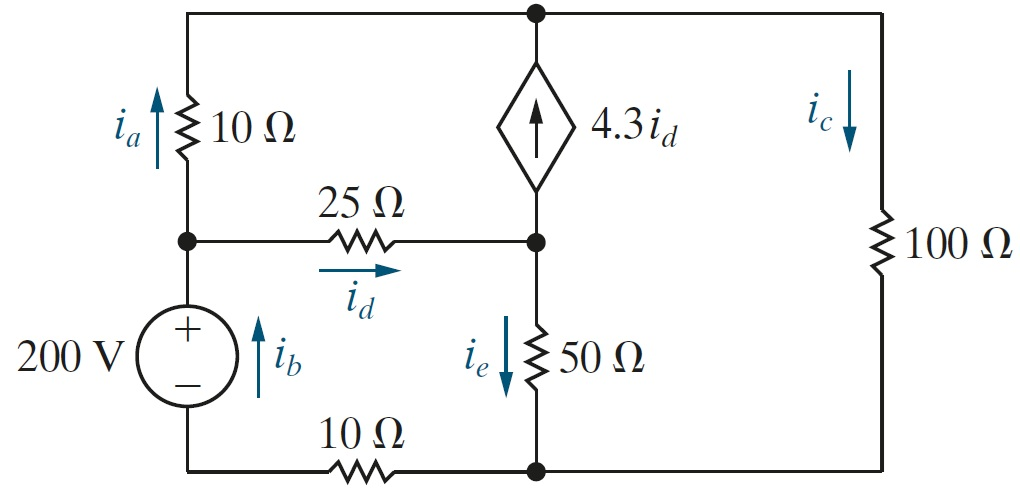
\includegraphics[width=0.6\textwidth]{Fig7.jpg} 
	\caption{Circuit for Problem~\ref{pb:p7}.}
	\label{fig:mesh1}
\end{figure}

\noindent\makebox[\linewidth]{\color{rouge_poly}{\rule{\textwidth}{1.3pt}}}

\begin{solprob} \text{}\\
    (a) Let's begin by writing the mesh equations:
    \[\text{Mesh 1: } -200 + 25(i_2-i_1)+50(i_2-i_3) + 10i_1 = 0\]
    \[200 = 25i_2 - 25i_1 + 50i_2 - 50i_3 + 10i_2\]
    \[200 = 85i_2-25i_1-50i_3\]
    \[\text{Supermesh: } 10i_1+100i_3+50(i_3-i_2)+25(i_1-i_2) = 0\]
    \[10i_1+100i_3+50i_3-50i_2+25i_1-25i_2=0\]
    \[35i_1-75i_2+150i_3 = 0\]
    \[i_2 = \frac{35i_1+150i_3}{75}\]
    Now, let's add a KCL to solve.
    \[i_d=i_e+4.3i_d \implies i_2-i_1=i_2-i_3+4.3(i_2-i_1)\implies i_3 = 4.3i_2 - 3.3i_1\]
    Now, sub in the supermesh into KCL to get $i_3$ in terms of $i_1$:
    \[i_3 = 4.3(\frac{35i_1+150i_3}{75})-3.3i_1\]
    \[i_3 = (\frac{150.5i_1+645i_3}{75})-3.3i_1\]
    \[7.6i_3 = 1.2933i_1\]
    \[i_3 = 0.170i_1\]
    Substitute this back into the supermesh equation:
    \[i_2 = \frac{35i_1 + 150(0.170i_1)}{75} = \frac{35i_1+25.526i_1}{75} = 0.807i_1\]
    Now, substitute this back into Mesh 1 equation to solve for $i_1$:
    \[200 = 85(0.807i_1)-50(0.170i_1)-25i_1\]
    \[200 = 68.5961i_1-8.5i_1-25i_1\]
    \[200 = 35.095i_1\]
    \[i_1 = 5.7\text{ A}\]
    Now, solve for remaining mesh currents.
    \[i_2 = 0.807(5.7) = 4.60 \text{ A}\]
    \[i_3 = 0.170(5.7) = 0.969\text{ A}\]
    Now solve for individual wire currents.
    \[i_a = i_1 = 5.70 \text{ A}\]
    \[i_b = i_2 = 4.60 \text{ A}\]
    \[i_c = i_3 = 0.969 \text{ A}\]
    \[i_d = i_2-i_1 = -1.1 \text{ A}\]
    \[i_e = i_2-i_3 = 3.63 \text{ A}\]
    (b) Let's calculate the total power developed vs total power dissipated.  Let's begin by calculating the power supplied from the sources:
    \[P_\text{src} = -vi = -(200)(4.60) = -920 \text{ W}\]
    To calculate the current in the dependent source, let's make a mesh current equation for the top mesh, using $V_o$ as the voltage across the CCCS.
    \[V_o + 10i_a +25(i_1-i_2) = 0 \implies V_o = -10(5.69) - 25(5.70-4.60) = -84.5 V\]
    \[P_\text{dep} = -V_o(4.3i_d) = -(-84.5)(4.3(-1.1)) = -399.685 \text{ W}\]
    \[\text{Total power supplied: } -920 - 399.685 = -1319.685 \text{ W}\]
    Now, let's calculate the power consumed by the resistors
    \[V_a = i_a^2R = (5.70)^2(10) = 324.9 \text{ W}\]
    \[V_b = i_b^2R = (4.60)^2(10) = 211.6 \text{ W}\]
    \[V_c = i_c^2R = (0.969)^2(100) = 93.8961 \text{ W}\]
    \[V_d = i_d^2R = (-1.1)^2(25) = 30.25 \text{ W}\]
    \[V_e = i_e^2R =  (3.63)^2(50) = 658.845 \text{ W}\]
    \[\text{Total power absorbed: } 324.9+211.6+93.8961+30.25+658.845 = 1319.4911 \text{ W}\]
    \[\therefore \text{Total power supplied}\approx \text{Total power absorbed}\]
\end{solprob}

\noindent\makebox[\linewidth]{\color{rouge_poly}{\rule{\textwidth}{1.3pt}}}	
%%%%%%%%%%%%%%%%%%%%%%%%%%%%%%%%%%%%%%%%%%%%%%%%%%%%%%%%%%%%%%%%%%%%%%%%%%%%%%%%%%%%%%%%%%%%%%%%%%%%%%%%%%%%%%
%%%%%%%%%%%%%%%%%%%%%%%%%%%%%%%%%%%%%%%%%%%%%%%%%%%%%%%%%%%%%%%%%%%%%%%%%%%%%%%%%%%%%%%%%%%%%%%%%%%%%%%%%%%%%%
%%%%%%%%%%%%%%%%%%%%%%%%%%%%%%%%%%%%%%%%%%%%%%%%%%%%%%%%%%%%%%%%%%%%%%%%%%%%%%%%%%%%%%%%%%%%%%%%%%%%%%%%%%%%%%
%%%%%%%%%%%%%%%%%%%%%%%%%%%%%%%%%%%%%%%%%%%%%%%%%%%%%%%%%%%%%%%%%%%%%%%%%%%%%%%%%%%%%%%%%%%%%%%%%%%%%%%%%%%%%%
\vspace{-5mm}

%% Alex 7th ed P3.70
\begin{prob}\label{pb:p8}
	Write the node-voltage equations and determine the values of $V_1$ and $V_2$ in the circuit of Fig.~\ref{fig:node2}.
\end{prob}

\vspace{-5mm}

\begin{figure}[H]
	\centering
	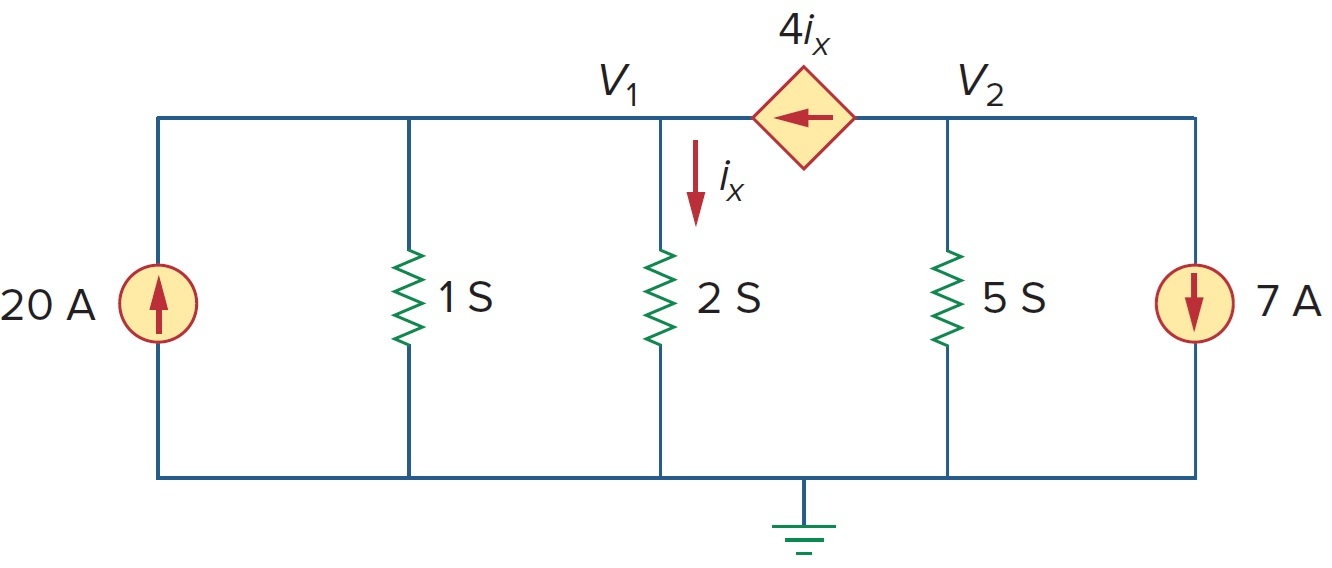
\includegraphics[width=0.6\textwidth]{Fig9.jpg} 
	\caption{Circuit for Problem~\ref{pb:p8}.}
	\label{fig:node2}
\end{figure}

\noindent\makebox[\linewidth]{\color{rouge_poly}{\rule{\textwidth}{1.3pt}}}

\begin{solprob} \text{}\\
    First things first, I began by converting the conductance units to ohms. Let's begin by writing the constraint equation:
    \[4I_x = \frac{V_1}{2}\]
    \[I_x = 2V_1\]
    Now, lets write the node voltage equations:
    \[-20+\frac{V_1}{1}+\frac{V_1}{0.5}-4I_x = 0\]
    \[-20+V_1+2V_1-8V_1 = 0\]
    \[20 = -5V_1\]
    \[V_1 = -4\text{ V}\]
    Now, let's write the other node equation:
    \[7+\frac{V_2}{0.2}+4I_x = 0\]
    \[7+5V_2+8V_1 = 0\]
    \[5V_2 = -7-8(-4)\]
    \[V_2 = 5\text{ V}\]
\end{solprob}

\noindent\makebox[\linewidth]{\color{rouge_poly}{\rule{\textwidth}{1.3pt}}}	
%%%%%%%%%%%%%%%%%%%%%%%%%%%%%%%%%%%%%%%%%%%%%%%%%%%%%%%%%%%%%%%%%%%%%%%%%%%%%%%%%%%%%%%%%%%%%%%%%%%%%%%%%%%%%%
%%%%%%%%%%%%%%%%%%%%%%%%%%%%%%%%%%%%%%%%%%%%%%%%%%%%%%%%%%%%%%%%%%%%%%%%%%%%%%%%%%%%%%%%%%%%%%%%%%%%%%%%%%%%%%
%%%%%%%%%%%%%%%%%%%%%%%%%%%%%%%%%%%%%%%%%%%%%%%%%%%%%%%%%%%%%%%%%%%%%%%%%%%%%%%%%%%%%%%%%%%%%%%%%%%%%%%%%%%%%%
%%%%%%%%%%%%%%%%%%%%%%%%%%%%%%%%%%%%%%%%%%%%%%%%%%%%%%%%%%%%%%%%%%%%%%%%%%%%%%%%%%%%%%%%%%%%%%%%%%%%%%%%%%%%%%
%% Alex 7th ed P3.80
\begin{prob}\label{pb:p9}
	Find the nodal voltages $v_1$ through $v_4$ in the circuit of Fig.~\ref{fig:node1}. 
	Check your solution with MATLAB/Simulink or PSpice.
\end{prob}

\begin{figure}[H]
	\centering
	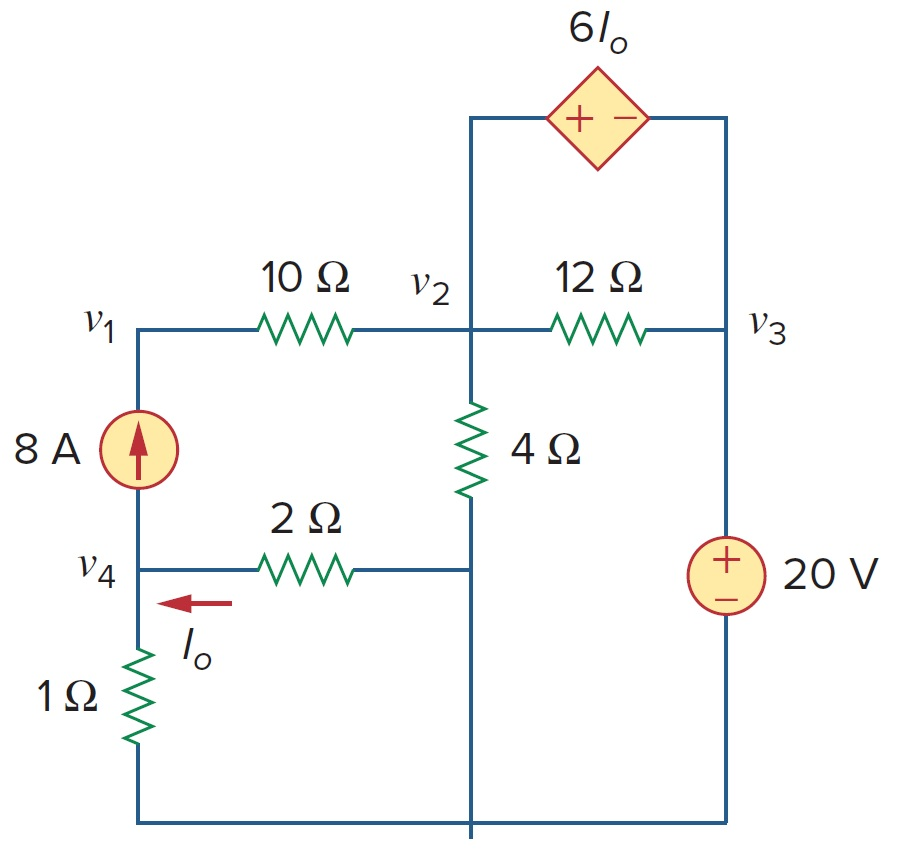
\includegraphics[width=0.56\textwidth]{Fig8.jpg} 
	\caption{Circuit for Problem~\ref{pb:p9}.}
	\label{fig:node1}
\end{figure}

\noindent\makebox[\linewidth]{\color{rouge_poly}{\rule{\textwidth}{1.3pt}}}

\begin{solprob} \text{}\\
    First, let's write the constraint equations.
    \[\text{First Constraint Equation: } V_2-V_3=6I_o\]
    \[\text{Second Constraint Equation: } I_o = \frac{V_4}{2}\]
    Now, let's write the first Node-Voltage equations:
    \[V_4 + 8 + \frac{V_4}{2} = 0 \implies \frac{3}{2}V_4 = -8 \implies V_4 = -5.33 \text{ V}\]
    We can substitute this value back into the second constraint equation to get $I_o$
    \[I_o = \frac{V_4}{2} = \frac{-5.33}{2} = -2.67\text{ A}\]
    Now, we can sub $I_o$ into the first equation.
    \[V_2-V_3=6(-2.67) = -16\]
    But here, we can see in the circuit that $V_3 = 20 \text{ V}$. We can use this value to solve for $V_2$:
    \[V_2 = -16+V_3 = -16 + 20 = 4 \text{ V}\]
    Now, we just need to solve for $V_1$, which we can get used the nodal voltage between $V_1$ and $V_2$:
    \[V_1-V_2 = 80\]
    \[V_1 = 80+V_2 = 80+4 = 84\text{ V}\]
    \[\therefore V_1 = 84\text{ V} \,\,\,\, V_2 = 4\text{ V}\,\,\,\,\ V_3 = 20\text{ V}\,\,\,\, V_4 = -5.33\text{ V}\]
    (b) PSpice circuit
    \begin{figure}[H]
    	\centering
    	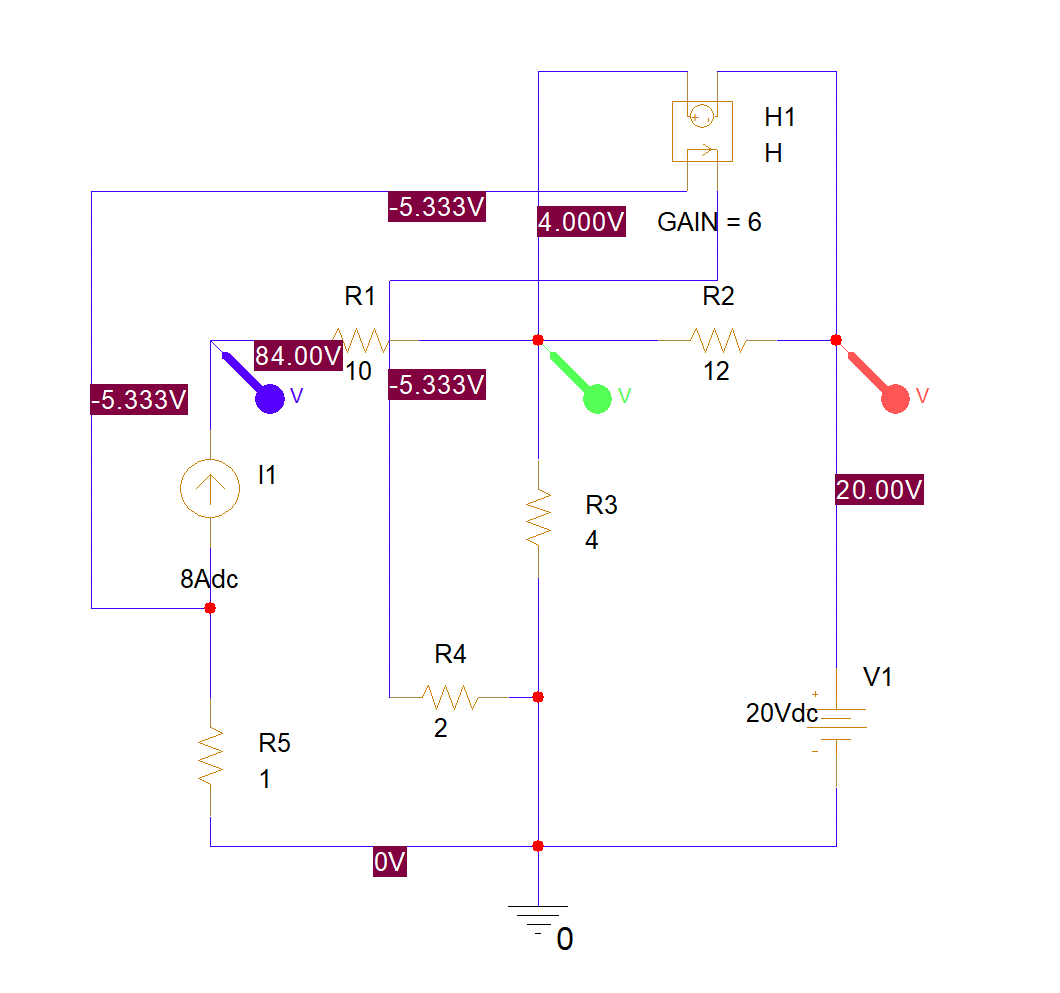
\includegraphics[width=0.56\textwidth]{PSPICE CIRCUIT Q9 HOMEWORK 2.png} 
    	\caption{Circuit for Problem~\ref{pb:p9}.}
    	\label{fig:node1}
    \end{figure}
\end{solprob}

\noindent\makebox[\linewidth]{\color{rouge_poly}{\rule{\textwidth}{1.3pt}}}	
%%%%%%%%%%%%%%%%%%%%%%%%%%%%%%%%%%%%%%%%%%%%%%%%%%%%%%%%%%%%%%%%%%%%%%%%%%%%%%%%%%%%%%%%%%%%%%%%%%%%%%%%%%%%%%
%%%%%%%%%%%%%%%%%%%%%%%%%%%%%%%%%%%%%%%%%%%%%%%%%%%%%%%%%%%%%%%%%%%%%%%%%%%%%%%%%%%%%%%%%%%%%%%%%%%%%%%%%%%%%%
%%%%%%%%%%%%%%%%%%%%%%%%%%%%%%%%%%%%%%%%%%%%%%%%%%%%%%%%%%%%%%%%%%%%%%%%%%%%%%%%%%%%%%%%%%%%%%%%%%%%%%%%%%%%%%
%%%%%%%%%%%%%%%%%%%%%%%%%%%%%%%%%%%%%%%%%%%%%%%%%%%%%%%%%%%%%%%%%%%%%%%%%%%%%%%%%%%%%%%%%%%%%%%%%%%%%%%%%%%%%%
%% Alex 7th ed P3.55
\begin{prob}\label{pb:p10}
	In the circuit of Fig.~\ref{fig:currents}, solve for $I_1$, $I_2$, and $I_3$.
\end{prob}

\begin{figure}[H]
	\centering
	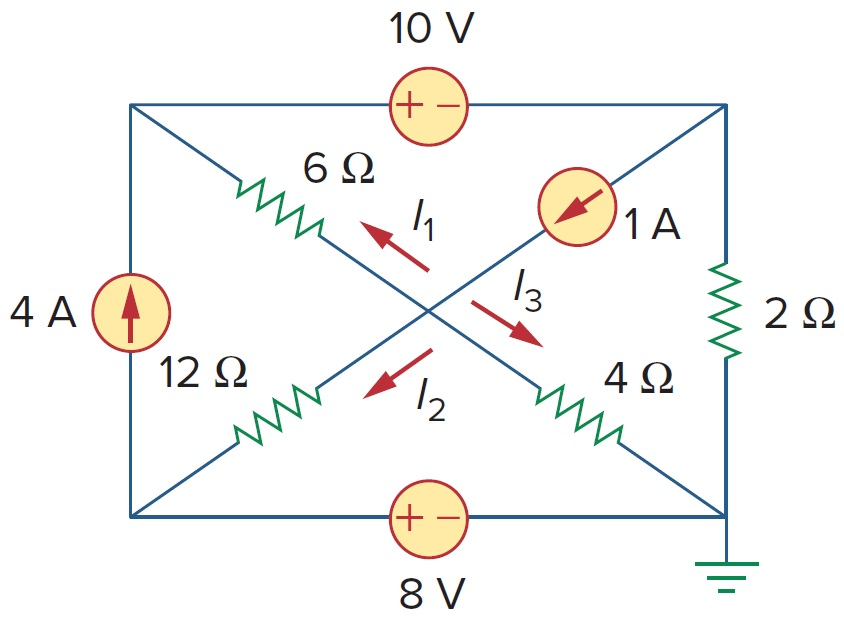
\includegraphics[width=0.56\textwidth]{Fig10.jpg} 
	\caption{Circuit for Problem~\ref{pb:p10}.}
	\label{fig:currents}
\end{figure}

\noindent\makebox[\linewidth]{\color{rouge_poly}{\rule{\textwidth}{1.3pt}}}

\begin{solprob} \text{}\\
    Let's use the mesh-current method. If we label the top mesh as $i_1$, right as $i_2$, bottom as $i_3$, left as $i_4$, we can immediately tell that $i_4 = 4$A, since we must include that current source in the the mesh. Let me also write a KCL equation:
    \[\text{KCL: }i_1 = 1+i_2\]
    Now, let's write the supermesh for the 1A current source:
    \[\text{Supermesh: } 10+2i_2+4(i_2-i_3)+6(i_1-i_4)=0\]
    Also, we can write a mesh equation for the bottom Mesh 3:
    \[\text{Mesh 3: } -8 + 4(i_3-i_2)+12(i_3-i_4)=0\]
    Let's use this equation to solve for $i_2$ in terms of $i_3$:
    \[-8+4i_3-4i_2+12i_3-12(4)=0\]
    \[-56+16i_3-4i_2=0\]
    \[-14+4i_3-i_2=0\]
    \[i_2=-14+4i_3\]
    We can sub this equation into KCL to be able to solve for $i_1$ in terms of $i_3$:
    \[i_1=1+(-14+4i_3)=-13+4i_3\]
    Now, lets take our supermesh equation and solve for $i_3$:
    \[10+2i_2+4(i_2-i_3)+6(i_1-i_4)=0\]
    \[10+2(-14+4i_3)+4(-14+4i_3-i_3)+6((-13+4i_3)-4)=0\]
    \[10-28+18i_3-56+12i_3-78+24i_3-24=0\]
    \[-176+44i_3=0\]
    \[i_3=\frac{176}{44}=4\text{ A}\]
    Now, we can solve for $i_1$ and $i_2$ using their respective equations:
    \[i_1=-13+4i_3=-13+4(4)=3\text{ A}\]
    \[i_2=-14+4(4)=2\text{ A}\]
    Now, we need to solve for actual currents using mesh currents:
    \[I_1 = i_1-i_4 = 3-4 = -1\text{ A}\]
    \[I_2=i_4-i_3=4-4 = 0\text{ A}\]
    \[I_3=i_3-i_2=4-2=2\text{ A}\]
\end{solprob}

\noindent\makebox[\linewidth]{\color{rouge_poly}{\rule{\textwidth}{1.3pt}}}	
%%%%%%%%%%%%%%%%%%%%%%%%%%%%%%%%%%%%%%%%%%%%%%%%%%%%%%%%%%%%%%%%%%%%%%%%%%%%%%%%%%%%%%%%%%%%%%%%%%%%%%%%%%%%%%
%%%%%%%%%%%%%%%%%%%%%%%%%%%%%%%%%%%%%%%%%%%%%%%%%%%%%%%%%%%%%%%%%%%%%%%%%%%%%%%%%%%%%%%%%%%%%%%%%%%%%%%%%%%%%%
%%%%%%%%%%%%%%%%%%%%%%%%%%%%%%%%%%%%%%%%%%%%%%%%%%%%%%%%%%%%%%%%%%%%%%%%%%%%%%%%%%%%%%%%%%%%%%%%%%%%%%%%%%%%%%
%%%%%%%%%%%%%%%%%%%%%%%%%%%%%%%%%%%%%%%%%%%%%%%%%%%%%%%%%%%%%%%%%%%%%%%%%%%%%%%%%%%%%%%%%%%%%%%%%%%%%%%%%%%%%%
%% Alex 7th ed P3.62
\begin{prob}\label{pb:p11}
	Use mesh analysis to find the mesh currents $i_1$, $i_2$, and $i_3$ in the network of Fig.~\ref{fig:mesh2}.
\end{prob}

\begin{figure}[H]
	\centering
	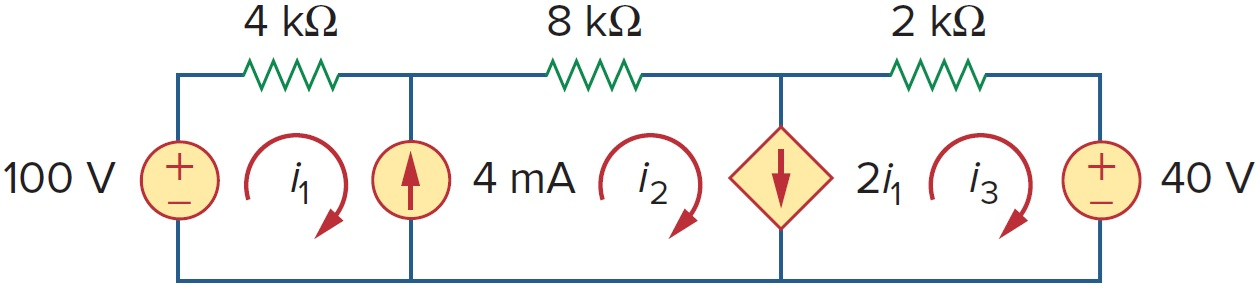
\includegraphics[width=0.76\textwidth]{Fig11.jpg} 
	\caption{Network for Problem~\ref{pb:p11}.}
	\label{fig:mesh2}
\end{figure}

\noindent\makebox[\linewidth]{\color{rouge_poly}{\rule{\textwidth}{1.3pt}}}

\begin{solprob} \text{}\\
    Let's begin by writing the supermesh equation:
    \[-100+4i_1+8i_2+2i_3+40=0\]
    \[-60+4i_1+8i_2+2i_3=0\]
    \[-30+2i_1+4i_2+i_3=0\]
    Now, let's write 2 KCL equations for the circuit:
    \[\text{KCL 1: } i_1+4=i_2 \implies i_1=i_2-4\]
    \[\text{KCL 2: } i_2=2i_1+i_3 \implies i_2=2(i_2-4)+i_3 \implies i_2=2i_2-8+i_3 \implies i_3=8-i_2\]
    Now, substitute the KCL equations into the supermesh equation:
    \[-30+2(i_2-4)+4i_2+(8-i_2)=0\]
    \[-30+2i_2-8+4i_2+8-i_2=0\]
    \[5i_2=30\]
    \[i_2=6.0 \text{ mA}\]
    Now solve for the rest of the mesh currents:
    \[i_1=i_2-4=6-4=2.0 \text{ mA}\]
    \[i_3=8-i_2=8-6=2\text{ mA}\]
\end{solprob}

\noindent\makebox[\linewidth]{\color{rouge_poly}{\rule{\textwidth}{1.3pt}}}	
%%%%%%%%%%%%%%%%%%%%%%%%%%%%%%%%%%%%%%%%%%%%%%%%%%%%%%%%%%%%%%%%%%%%%%%%%%%%%%%%%%%%%%%%%%%%%%%%%%%%%%%%%%%%%%
%%%%%%%%%%%%%%%%%%%%%%%%%%%%%%%%%%%%%%%%%%%%%%%%%%%%%%%%%%%%%%%%%%%%%%%%%%%%%%%%%%%%%%%%%%%%%%%%%%%%%%%%%%%%%%
%%%%%%%%%%%%%%%%%%%%%%%%%%%%%%%%%%%%%%%%%%%%%%%%%%%%%%%%%%%%%%%%%%%%%%%%%%%%%%%%%%%%%%%%%%%%%%%%%%%%%%%%%%%%%%
%%%%%%%%%%%%%%%%%%%%%%%%%%%%%%%%%%%%%%%%%%%%%%%%%%%%%%%%%%%%%%%%%%%%%%%%%%%%%%%%%%%%%%%%%%%%%%%%%%%%%%%%%%%%%%	
% Nilsson 12th ed P4.28
\begin{prob}\label{pb:p12}
	Use the node-voltage method to find the power developed by the voltage-controlled current source in the circuit of Fig.~\ref{fig:vc_cs}.
\end{prob}

\begin{figure}[H]
	\centering
	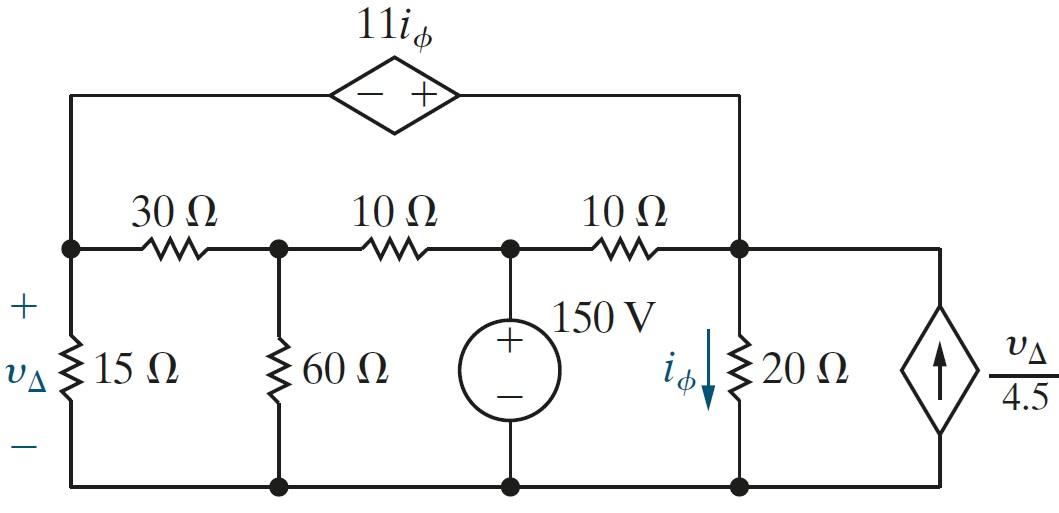
\includegraphics[width=0.6\textwidth]{Fig12.jpg} 
	\caption{Circuit for Problem~\ref{pb:p12}.}
	\label{fig:vc_cs}
\end{figure}

\noindent\makebox[\linewidth]{\color{rouge_poly}{\rule{\textwidth}{1.3pt}}}

\begin{solprob} \text{}\\
    Let's begin by writing the node-voltage equations for this circuit:
    \[\text{First equation: } \frac{V_1}{15}+\frac{V_1-V_2}{30}+\frac{V_3-150}{10}+\frac{V_3}{20}-\frac{V_1}{4.5} = 0\]
    \[\text{Second Equation: } \frac{V_2-V_1}{30}+\frac{V_2}{60}+\frac{V_2-150}{10}=0\]
    Let's take this second equation and solve for $V_2$ in terms of $V_1$:
    \[2(V_2-V_1)+V_2+6(V_2-150)=0\]
    \[2V_2-2V_1+V_2+6V_2-900=0\]
    \[9V_2=2V_1+900\]
    \[V_2=\frac{2}{9}V_1+100\]
    Now, let's write an equation for the supernode at the top of the circuit containing the CCVS:
    \[V_1+11i_\phi = V_3\]
    But we know that $i_\phi = \frac{V_3}{20}$:
    \[V_1+11(\frac{V_3}{20})=V_3\]
    \[V_1=\frac{9}{20}V_3\]
    \[V_3 = \frac{20}{9}V_1\]
    Now, sub these into the first mesh equation to solve for $V_1$:
    \[\frac{V_1}{15}+\frac{V_1-V_2}{30} + \frac{V_3-150}{10} + \frac{V_3}{20} - \frac{V_1}{4.5} = 0\]
    \[\]
\end{solprob}

\noindent\makebox[\linewidth]{\color{rouge_poly}{\rule{\textwidth}{1.3pt}}}	
%%%%%%%%%%%%%%%%%%%%%%%%%%%%%%%%%%%%%%%%%%%%%%%%%%%%%%%%%%%%%%%%%%%%%%%%%%%%%%%%%%%%%%%%%%%%%%%%%%%%%%%%%%%%%%
%%%%%%%%%%%%%%%%%%%%%%%%%%%%%%%%%%%%%%%%%%%%%%%%%%%%%%%%%%%%%%%%%%%%%%%%%%%%%%%%%%%%%%%%%%%%%%%%%%%%%%%%%%%%%%
%%%%%%%%%%%%%%%%%%%%%%%%%%%%%%%%%%%%%%%%%%%%%%%%%%%%%%%%%%%%%%%%%%%%%%%%%%%%%%%%%%%%%%%%%%%%%%%%%%%%%%%%%%%%%%
%%%%%%%%%%%%%%%%%%%%%%%%%%%%%%%%%%%%%%%%%%%%%%%%%%%%%%%%%%%%%%%%%%%%%%%%%%%%%%%%%%%%%%%%%%%%%%%%%%%%%%%%%%%%%%	
%% Dorf 9th ed P4.7-15
\begin{prob}\label{pb:p13}
	Determine the values of the mesh currents $i_1$ and $i_2$ for the circuit shown in Fig.~\ref{fig:mesh3}.
\end{prob}

\begin{figure}[H]
	\centering
	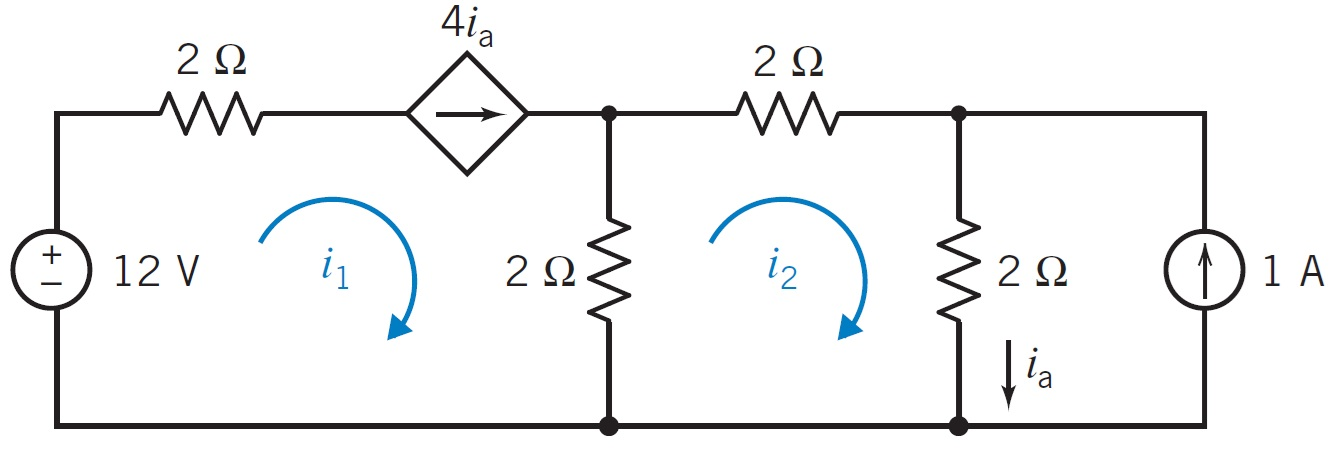
\includegraphics[width=0.6\textwidth]{Fig13.jpg} 
	\caption{Circuit for Problem~\ref{pb:p13}.}
	\label{fig:mesh3}
\end{figure}

\noindent\makebox[\linewidth]{\color{rouge_poly}{\rule{\textwidth}{1.3pt}}}

\begin{solprob} \text{}\\
    Let's begin by writing the the mesh equation, a KCL and a constraint equation:
    \[\text{Mesh 1: } 2(i_2-i_1)+2i_2+2(i_2+1)=0\]
    \[\text{KCL: } i_2+1=i_a \implies i_2 = i_a-1\]
    \[\text{Constraint: } i_1=4i_a\]
    Let's take the mesh equation and solve for $i_a$.
    \[2i_2-2i_1+2i_2+2i_2+2 = 0\]
    \[6i_2-2i_1+2=0\]
    Now, sub in the other equations into $i_2$ and $i_1$:
    \[6(i_a-1)-2(4i_a)+2=0\]
    \[6i_a-6-8i_a+2=0\]
    \[-2i_a-4=0\]
    \[i_a=-2 \text{ A}\]
    Now, solve for the remaining currents:
    \[i_1=4i_a=4(-2)=-8 \text{ A}\]
    \[i_2=i_a-1=-2-1=-3 \text{ A}\]
\end{solprob}

\noindent\makebox[\linewidth]{\color{rouge_poly}{\rule{\textwidth}{1.3pt}}}	
%%%%%%%%%%%%%%%%%%%%%%%%%%%%%%%%%%%%%%%%%%%%%%%%%%%%%%%%%%%%%%%%%%%%%%%%%%%%%%%%%%%%%%%%%%%%%%%%%%%%%%%%%%%%%%
%%%%%%%%%%%%%%%%%%%%%%%%%%%%%%%%%%%%%%%%%%%%%%%%%%%%%%%%%%%%%%%%%%%%%%%%%%%%%%%%%%%%%%%%%%%%%%%%%%%%%%%%%%%%%%
%%%%%%%%%%%%%%%%%%%%%%%%%%%%%%%%%%%%%%%%%%%%%%%%%%%%%%%%%%%%%%%%%%%%%%%%%%%%%%%%%%%%%%%%%%%%%%%%%%%%%%%%%%%%%%
%%%%%%%%%%%%%%%%%%%%%%%%%%%%%%%%%%%%%%%%%%%%%%%%%%%%%%%%%%%%%%%%%%%%%%%%%%%%%%%%%%%%%%%%%%%%%%%%%%%%%%%%%%%%%%	
%% Nilsson 12th ed, P4.81
\begin{prob}\label{pb:p14}
	Find the Thévenin equivalent with respect to the terminals $a$ and $b$ in the circuit shown in Fig.~\ref{fig:thevencircuit}.
\end{prob}
\vspace{-4mm}
\begin{figure}[H]
	\centering
	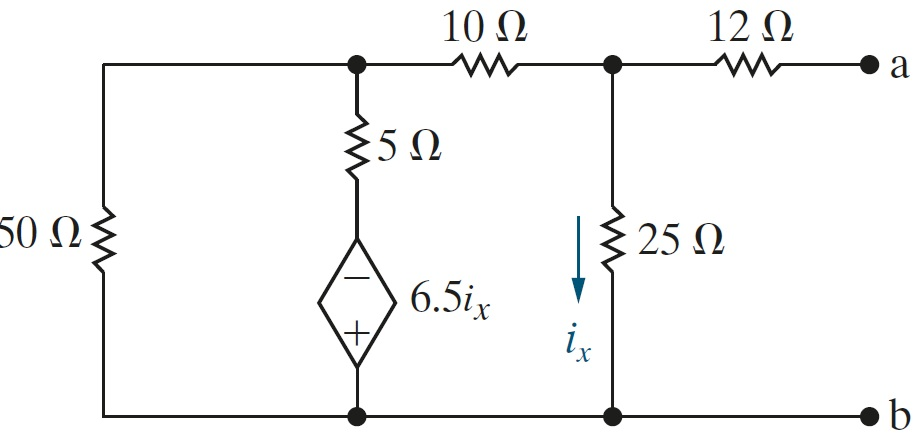
\includegraphics[width=0.56\textwidth]{Fig14.jpg} 
	\caption{Circuit for Problem~\ref{pb:p14}.}
	\label{fig:thevencircuit}
\end{figure}

\noindent\makebox[\linewidth]{\color{rouge_poly}{\rule{\textwidth}{1.3pt}}}

\begin{solprob} \text{}\\
    First, lets connect point a and point b using a 1 A test source.  Now, let's write node-voltage equations:
    \[\text{Equation 1: } \frac{V_1-V_2}{10}+\frac{V_1+6.5i_x}{5}+\frac{V_1}{50}=0\]
    \[\text{Equation 2: } \frac{V_2-V_1}{10}+\frac{V_2}{25}-1=0\]
    Let's also write a constraint equation for $i_x$:
    \[i_x=\frac{V_2}{25}\]
    Let's take Equation 1 and substitute in the constraint equation:
    \[\frac{V_1-V_2}{10}+\frac{V_1+6.5(\frac{V_2}{25})}{5}+\frac{V_1}{50}=0\]
    \[5(V_1-V_2)+10V_1+65(\frac{V_2}{25})+V_1=0\]
    \[5V_1-5V_2+10V_1+\frac{65}{25}V_2+V_1=0\]
    \[16V_1=2.4V_2\]
    \[V_1=0.15V_2\]
    Now, use this equation to substitute into the second equation: 
    \[5V_2-5V_1+2V_2-50=0\]
    \[5V_2-5(0.15V_2)+2V_2-50=0\]
    \[6.25V_2=50\]
    \[V_2=8 \text{ V}\]
    Now, solve for $V_1$:
    \[V_1=0.15(8)=1.2 \text{ V}\]
    Now, we need to calculate $V_\text{Th}$ and $R_\text{Th}$, we can do this by calculating the voltage difference between $V_2$ and $V_a$:
    \[V_\text{Th} = V_2+12(1) = 8+12 = 20\text{ V}\]
    \[R_\text{Th} = \frac{20}{1} = 20\,\Omega\]
\end{solprob}

\noindent\makebox[\linewidth]{\color{rouge_poly}{\rule{\textwidth}{1.3pt}}}	
%%%%%%%%%%%%%%%%%%%%%%%%%%%%%%%%%%%%%%%%%%%%%%%%%%%%%%%%%%%%%%%%%%%%%%%%%%%%%%%%%%%%%%%%%%%%%%%%%%%%%%%%%%%%%%
%%%%%%%%%%%%%%%%%%%%%%%%%%%%%%%%%%%%%%%%%%%%%%%%%%%%%%%%%%%%%%%%%%%%%%%%%%%%%%%%%%%%%%%%%%%%%%%%%%%%%%%%%%%%%%
%%%%%%%%%%%%%%%%%%%%%%%%%%%%%%%%%%%%%%%%%%%%%%%%%%%%%%%%%%%%%%%%%%%%%%%%%%%%%%%%%%%%%%%%%%%%%%%%%%%%%%%%%%%%%%
%%%%%%%%%%%%%%%%%%%%%%%%%%%%%%%%%%%%%%%%%%%%%%%%%%%%%%%%%%%%%%%%%%%%%%%%%%%%%%%%%%%%%%%%%%%%%%%%%%%%%%%%%%%%%%	
%% Nilsson 12th ed, P4.98
\begin{prob}\label{pb:p15}
	Use the principle of superposition to find the voltage $v$ in the circuit shown in Fig.~\ref{fig:superposition}.
\end{prob}
\vspace{-3mm}
\begin{figure}[H]
	\centering
	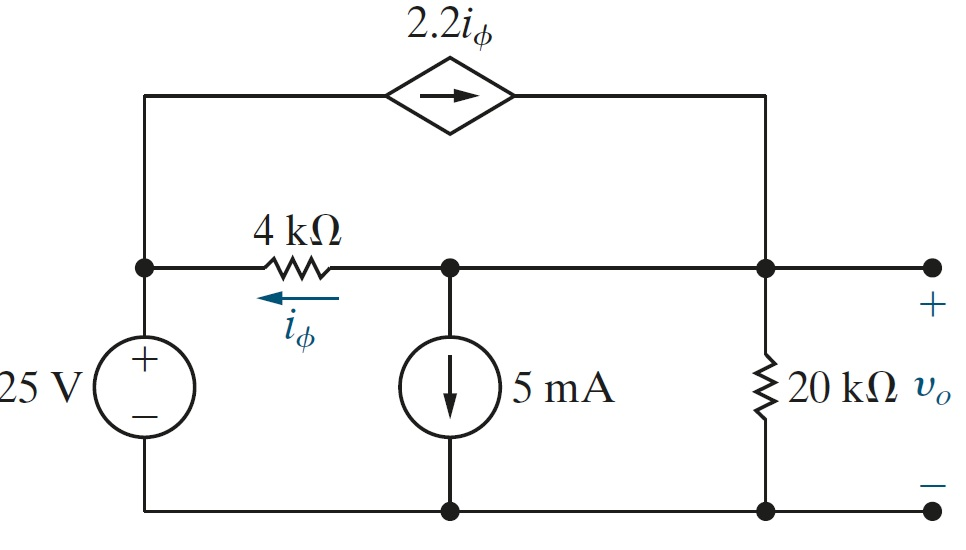
\includegraphics[width=0.54\textwidth]{Fig15.jpg} 
	\caption{Circuit for Problem~\ref{pb:p15}.}
	\label{fig:superposition}
\end{figure}

\noindent\makebox[\linewidth]{\color{rouge_poly}{\rule{\textwidth}{1.3pt}}}

\begin{solprob} \text{}\\
    Let's start with solving the circuit by opening the circuit, removing the current source. Now, let's solve for $V_o^\prime$:
    \[\text{Equation 1: }\frac{V_o^\prime-25}{4000}+\frac{V_o^\prime}{20000}-2.2i_\phi=0\]
    \[\text{Constraint Equation: } i_\phi = \frac{V_o^\prime-25}{4000}\]
    Now, solve for $V_o^\prime$:
    \[5V_o^\prime-125+V_o^\prime-44000i_\phi=0\]
    \[6V_o^\prime-125-44000(\frac{V_o^\prime-25}{4000})=0\]
    \[6V_o^\prime-125-11V_o^\prime+275=0\]
    \[5V_o^\prime=150\]
    \[V_o^\prime=30 \text{ V}\]
    Now, lets short circuit the circuit and remove the voltage sources, after adding the current sources back. Let's solve for $V_o^\text{$\prime\prime$}$:
    \[\text{Constraint: } i_\phi = \frac{V_o^\text{$\prime\prime$}}{4000}\]
    \[\text{Equation 1: } \frac{V_o^\text{$\prime\prime$}}{4000} + \frac{V_o^\text{$\prime\prime$}}{20000} + 0.005-2.2i_\phi=0\]
    \[5V_o^\text{$\prime\prime$}+V_o^\text{$\prime\prime$}+100-44000(\frac{V_o^\text{$\prime\prime$}}{4000})=0\]
    \[6V_o^\text{$\prime\prime$}+100-11V_o^\text{$\prime\prime$}=0\]
    \[5V_o^\text{$\prime\prime$}=100\]
    \[V_o^\text{$\prime\prime$}=20\text{ V}\]
    Now, lets calculate $V_o$'s actual value:
    \[V_o=V_o^\text{$\prime$} + V_o^\text{$\prime\prime$} = 30 + 20 = 50 \text{ V}\]
\end{solprob}

\noindent\makebox[\linewidth]{\color{rouge_poly}{\rule{\textwidth}{1.3pt}}}	
%%%%%%%%%%%%%%%%%%%%%%%%%%%%%%%%%%%%%%%%%%%%%%%%%%%%%%%%%%%%%%%%%%%%%%%%%%%%%%%%%%%%%%%%%%%%%%%%%%%%%%%%%%%%%%
%%%%%%%%%%%%%%%%%%%%%%%%%%%%%%%%%%%%%%%%%%%%%%%%%%%%%%%%%%%%%%%%%%%%%%%%%%%%%%%%%%%%%%%%%%%%%%%%%%%%%%%%%%%%%%
%%%%%%%%%%%%%%%%%%%%%%%%%%%%%%%%%%%%%%%%%%%%%%%%%%%%%%%%%%%%%%%%%%%%%%%%%%%%%%%%%%%%%%%%%%%%%%%%%%%%%%%%%%%%%%
%%%%%%%%%%%%%%%%%%%%%%%%%%%%%%%%%%%%%%%%%%%%%%%%%%%%%%%%%%%%%%%%%%%%%%%%%%%%%%%%%%%%%%%%%%%%%%%%%%%%%%%%%%%%%%	

%% Nilsson 12th ed, P4.91
\begin{prob}\label{pb:p16}
	The variable resistor $R_L$ in the circuit shown in Fig.~\ref{fig:maxpower} is adjusted for maximum power transfer to $R_L$.
	\begin{enumerate}[label=\textbf{(\alph*)}]
		\item Find the numerical value of $R_L$.
		\item Find the maximum power transferred to $R_L$.
	\end{enumerate}
\end{prob}
\vspace{-2mm}
\begin{figure}[H]
	\centering
	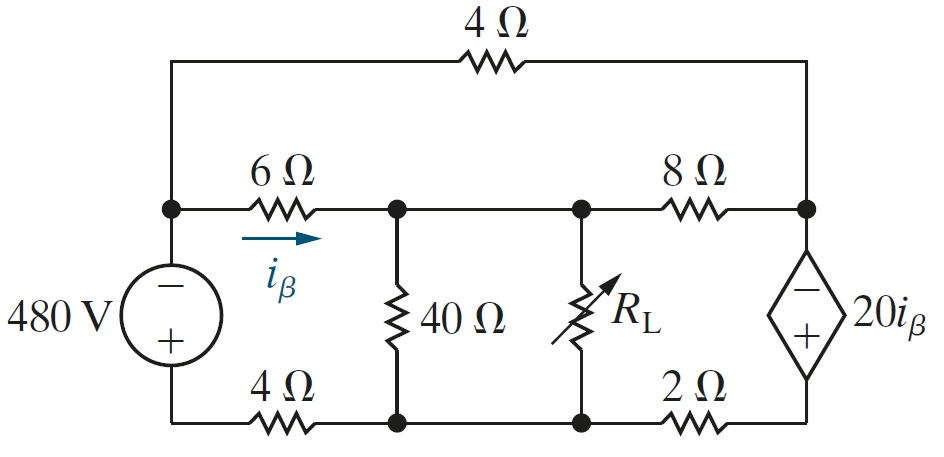
\includegraphics[width=0.6\textwidth]{Fig16.jpg} 
	\caption{Circuit for Problem~\ref{pb:p16}.}
	\label{fig:maxpower}
\end{figure}

\noindent\makebox[\linewidth]{\color{rouge_poly}{\rule{\textwidth}{1.3pt}}}

\begin{solprob} \text{}\\
    (a)Let's begin by opening the circuit on $R_L$, and writing mesh equations if the top mesh is 1, bottom left mesh is 2, and bottom left mesh is 3:
    \[\text{Constraint: } i_\beta=i_2-i_1\]
    \[\text{Mesh 1: }6(i_1-i_2)+4i_1+8(i_1-i_3)=0\]
    \[\text{Mesh 2: }480+6(i_2-i_1)+40(i_2-i_3)+4i_2=0\]
    \[\text{Mesh 3: }-20i_\beta + 2i_3+40(i_3-i_2)+8(i_3-i_1)=0\]
    Expand Mesh 3 Equation to solve for $i_1$ in terms of $i_2$ and $i_3$:
    \[-20i_2+20i_1+2i_3+40i_3-40i_2+8i_3-8i_1=0\]
    \[12i_1-60i_2+50i_3=0\]
    \[12i_1=60i_2-50i_3\]
    \[i_1=5i_2-\frac{50}{12}i_3\]
    Now, expand Mesh 1, and substitute in this $i_1$ equation to solve for $i_2$ in terms of $i_3$:
    \[6i_1-6i_2+4i_1+8i_1-8i_3=0\]
    \[18i_1-6i_2-8i_3=0\]
    \[18(5i_2-\frac{50}{12}i_3)-6i_2-8i_3=0\]
    \[90i_2-75i_3-6i_2-8i_3=0\]
    \[84i_2-83i_3=0\]
    \[i_2=\frac{83}{84}i_3\]
    Now, let's substitute this value back into our $i_1$ equation:
    \[i_1=5i_2-\frac{50}{12} = 5(\frac{83}{84}i_3)-\frac{50}{12}i_3 = \frac{415}{84}i_3-\frac{350}{84}i_3=\frac{65}{84}i_3\]
    Now take these two equations and sub into Mesh 2 equation:
    \[480+6i_2-6i_1+40i_2-40i_3+4i_2=0\]
    \[480+50i_2+6i_2-40i_3=0\]
    \[480+\frac{4150}{84}i_3-\frac{390}{84}-40i_3=0\]
    \[4.76i_3=-480\]
    \[i_3=-100.8\text{ A}\]
    Now, solve for the other 2 mesh currents:
    \[i_1=\frac{65}{84}(-100.8)=-78 \text{ A}\]
    \[i_2=\frac{83}{84}(-100.8)=-99.6 \text{ A}\]
    We can also solve for $V_\text{Th}$:
    \[V_\text{Th} = 40(i_1-i_3) = 40(-78-(-100.8))=48 \text{ V}\]
    Now, let's go back to the original circuit and short circuit the $R_L$ wire.  Lets begin by writing the mesh equations again:
    \[\text{Mesh 1: } 8(i_1-i_3)+4i_1+6(i_1-i_2)=0\]
    \[\text{Mesh 2: } 480+6(i_2-i_1)+4i_2=0\]
    \[\text{Mesh 3: } -20i_\beta + 2i_3+8(i_3-i_1)=0\]
    We use the same constraint equation $i_\beta=i_2-i_1$:
    Let's expand and solve for $i_1$ as we did before:
    \[-20i_2+20i_1+2i_3+8i_3-8i_1=0\]
    \[12i_1-20i_2+10i_3=0\]
    \[i_2=\frac{12}{20}i_1+0.5i_3\]
    Now sub this back into the expanded version of mesh 1:
    \[8i_1-8i_3+4i_1+6i_1-6i_2=0\]
    \[18i_1-6i_2-8i_3=0\]
    \[18i_1-6(\frac{12}{20}i_1+0.5i_3)-8i_3=0\]
    \[18i_1 - \frac{72}{20}i_1-3i_3-8i_3=0\]
    \[14.4i_1-11i_3=0\]
    \[i_3=\frac{14.4}{11}i_1\]
    Now, substitute this back into the $i_2$ equation:
    \[i_2=\frac{12}{20}i_1+0.5i_3=\frac{12}{20}i_1+\frac{14.4}{22}i_1=\frac{132}{220}i_1+\frac{144}{220}i_1=\frac{276}{220}i_1\]
    Now solve for $i_1$ in mesh 2 equation:
    \[480+6i_2-6i_1+4i_2=0\]
    \[480+10i_2-6i_1=0\]
    \[480+\frac{276}{22}i_1-6i_1=0\]
    \[480=-\frac{144}{22}i_1\]
    \[i_1=-73.33 \text{ A}\]
    Now solve for the remaining mesh currents:
    \[i_2=\frac{276}{220}i_1=\frac{276}{220}(-73.33) = -92 \text{ A}\]
    \[i_3 = \frac{14.4}{11}i_1 = \frac{14.4}{11}(-73.33) = -96 \text{ A}\]
    Now, we can calculate the short circuit current:
    \[i_\text{sc} = i_2-i_3=-92-(-96)=4 \text{ A}\]
    And now we can calculate the value of $R_L$:
    \[R_\text{Th} = \frac{V_\text{Th}}{i_\text{sc}} = \frac{48}{4} = 12\Omega = R_L\]
    (b) To calculate the maximum power transferred, we simply use the values from part (a):
    \[p_\text{max} = \frac{(V_\text{Th})^2}{4R_\text{Th}} = \frac{(48)^2}{4(12)} = 48 \text{ W}\]
\end{solprob}

%\noindent\makebox[\linewidth]{\color{rouge_poly}{\rule{\textwidth}{1.3pt}}}	
%%%%%%%%%%%%%%%%%%%%%%%%%%%%%%%%%%%%%%%%%%%%%%%%%%%%%%%%%%%%%%%%%%%%%%%%%%%%%%%%%%%%%%%%%%%%%%%%%%%%%%%%%%%%%%
%%%%%%%%%%%%%%%%%%%%%%%%%%%%%%%%%%%%%%%%%%%%%%%%%%%%%%%%%%%%%%%%%%%%%%%%%%%%%%%%%%%%%%%%%%%%%%%%%%%%%%%%%%%%%%
%%%%%%%%%%%%%%%%%%%%%%%%%%%%%%%%%%%%%%%%%%%%%%%%%%%%%%%%%%%%%%%%%%%%%%%%%%%%%%%%%%%%%%%%%%%%%%%%%%%%%%%%%%%%%%
%%%%%%%%%%%%%%%%%%%%%%%%%%%%%%%%%%%%%%%%%%%%%%%%%%%%%%%%%%%%%%%%%%%%%%%%%%%%%%%%%%%%%%%%%%%%%%%%%%%%%%%%%%%%%%	 
\end{document}


